\documentclass[a4,12pt,twoside]{article}
\newif\ifRR
\RRtrue % \RRfalse or \RRtrue

\ifRR
\usepackage[a4paper]{geometry}
\usepackage{RR}
\graphicspath{{../etc/rr-sty/}}
\else
\usepackage[top=1.5cm,right=4cm,bottom=2cm,left=1.5cm]{geometry}
\fi
\usepackage[T1]{fontenc} \usepackage[utf8]{inputenc}
\usepackage{authblk}
\usepackage{graphicx} 
\usepackage{hyperref}
\usepackage{amsmath}\usepackage{amsfonts}
\newcommand{\deq}{\stackrel {\rm def}{=}}
\newcommand{\eqline}[1]{\\\centerline{$#1$}\\} 
\newcommand{\hr}{\\---------------------------------------------------}
\newcommand{\tab}{\\\hspace{5mm}} 

\usepackage{color}
\definecolor{fred}{RGB}{32,64,128}\newcommand{\fred}[1]{{\color{fred}{{\tt @fred:} #1}}}
\definecolor{thalita}{RGB}{51, 153, 255}\newcommand{\thalita}[1]{{\color{thalita}{{\tt @thalita:} #1}}}
\definecolor{vthierry}{RGB}{80,0,120}\newcommand{\vthierry}[1]{{\color{vthierry}{{\tt @vthierry:} #1}}}
\definecolor{xavier}{RGB}{42,120,42}\newcommand{\xavier}[1]{{\color{xavier}{{\tt @xavier:} #1}}}

\ifRR
\RRNo{9100}
\RRdate{October 2017}
\RRauthor{\thanks[affil]{Mnemosyne team, INRIA Bordeaux}
Thierry Vi\'eville \thanksref{affil} \and
Xavier Hinaut \thanksref{affil} \and
Thalita F. Drumond \thanksref{affil} \and
Fr\'ed\'eric Alexandre \thanksref{affil}}
\authorhead{Alexandre \& Drumond \& Hinault \& Vi\'eville}
\RRtitle{Estimation des poids d'un réseau récurrent \\ par ajustement rétroactif}
\RRetitle{Recurrent neural network weight estimation \\ through backward tuning}
\titlehead{Backward tuning}
\RRresume{Nous considérons une formulation alternative de l'estimation du poids dans les réseaux récurrents, proposant une notation integrant une grande quantité d'unités de réseau récurrentes qui aide à formuler ce problème d'estimation. Réutilisant un «bon vieux» principe de la théorie du contrôle, amélioré ici à l'aide d'une heuristique de stabilisation numérique rétroactive, nous obtenons une estimation distribuée du 2ème ordre, numériquement stable et plutôt efficace, sans aucun méta-paramètre à ajuster. La relation avec les techniques existantes est discutée à chaque étape. La méthode proposée est validée en utilisant des tâches d'ingénierie inverse.}
\RRabstract{We consider another formulation of weight estimation in recurrent networks, proposing a notation for a large amount of recurrent network units that helps formulating the estimation problem. Reusing a ``good old'' control-theory principle, improved here using a backward-tuning numerical stabilization heuristic, we obtain a numerically stable and rather efficient second-order and distributed estimation, without any meta-parameter to adjust. The relation with existing technique is discussed at each step. 
The proposed method is validated using reverse engineering tasks.

}
\RRmotcle{réseaux récurrents, apprentissage automatique, ajustement rétroactif}
\RRkeyword{recurrent network, machine learning, backward tuning}
\RRprojet{Mnemosyne}
\RCBordeaux
\fi

\begin{document}
\ifRR
\makeRR 
\else
\title{Recurrent neural network weight estimation \\ though backward tuning}
\author[1]{Fr\'ed\'eric Alexandre}
\author[1]{Thalita F. Drumond}
\author[1]{Xavier Hinaut}
\author[1]{Thierry Vi\'eville}
\affil[1]{Mnemosyne team, INRIA Bordeaux}
\maketitle
\begin{abstract}We consider another formulation of weight estimation in recurrent networks, proposing a notation for a large amount of recurrent network units that helps formulating the estimation problem. Reusing a ``good old'' control-theory principle, improved here using a backward-tuning numerical stabilization heuristic, we obtain a numerically stable and rather efficient second-order and distributed estimation, without any meta-parameter to adjust. The relation with existing technique is discussed at each step. 
The proposed method is validated using reverse engineering tasks.

\end{abstract}
\fi
\iffalse
\fi
\section{Introduction}

Artificial neural networks can be considered as discrete-time
dynamical systems, performing input-output computation, at the higher
level of generality \cite{siegelmann_turing_1991}. The computation is
defined by the adjustment of the network connection weights and
related parameters\footnote{Other network parameters include the unit
  leak, intrisic plasticity, parameters of the non-linearity (or
  activation function). However, in this paper we are going to use a
  notation allowing us to consider all these parameters as connection
  weights for an extended set of state variables.} In fact, only specific
feed-forward or recurrent architectures are considered in practice,
because of network parameters estimation, as reviewed now.

In the artificial neural network literature, feed-forward networks
parameter learning is a rather well-solved problem.  For instance, the
back-propagation algorithms, based on specific architectures of
multi-layer feed-forward networks, allows one to propose well-defined
implementation \cite{amit:89}, though it has been shown at the
theoretical and empirical levels that "shallow" architectures are
inefficient for representing complex functions \cite{Poggio2017,bengio-lecun:07},
or at the cost of huge network sizes as in, e.g., extreme learning
\cite{HUANG2006489}. 

Deep-networks are specific feed-forward architectures
\cite{bengio-lecun:07} which can have very impressive performances,
e.g.  \cite{farabet_learning_2013}. The key idea
\cite{hstad_power_1991} is that, at least for threshold units with
positive weights, reducing the number of layers induces an exponential
complexity increase for the same input/output function. On the
reverse, it is a reasonable assumption, numerically verified, that
increasing the number of layers yields a input/output function compact
representation (in the sense of \cite{hstad_power_1991}, i.e., as a
hierachical composition of local functions). One drawback is related
to weights supervised learning in deeper layers, since readout layers
may over-fit the learning set, the remedy being to apply unsupervised
learning on deeper layers (see \cite{Bengio:2009} for an
introduction). This problem is highly reduced with specific
architectures such as CNN \cite{Lecun1998Gradient}.

It also remains restrictive by the fact that the architecture is
mainly a pipe-line including some parallel tracks or short-cuts, while each layer is
a feed-forward network (e.g. a convolutional neural layers) or with a
very specific recurrent connectivity (e.g., restrained Boltzman
machines).  Starting with LeNet-5 \cite{Lecun1998Gradient}, different
successful architectures in term of performance have been proposed (e.g.,
AlexNet\cite{Krizhevsky2012Imagenet}, ZF net
\cite{Zeiler2014Visualizing}, Overfeat \cite{Sermanet2013Overfeat},
VGG \cite{Simonyan2015Very}, GoogLeNet \cite{Szegedy2014Going},
Inspection \cite{Szegedy2016Inception}, residual nets
\cite{He2016Deep}).

In the brain, more general architectures exist (e.g.  with shortcuts
between deeper and lower layers, as it happens in the visual system
regarding the thalamus \cite{citeulike:1590763}) and each layer is a
more general recurrent network (e.g., with short and long range
horizontal connections). Breaking this pipe-line architecture may
overcome the problem of deeper layer weight adjustment, and the need
of huge architecture in order to obtain high performances. 
This is the origin of the present work.

Feed-forward networks are obviously far from the computational
capacity of recurrent networks
\cite{Goodfellow2016Deep,Schmidhuber:2015,cessac_view_2010}.
Therefore, specific multi-layer architectures with recurrent links
within a layer and specific forward/backward connections between
layers have been proposed instead. The first dynamic neural model, the
model by Hopfield \cite{hopfield:82}, or its randomized version as a
Boltzman machine, was very specific. For such specific networks, such
as bidirectional associative memory
\cite{Acevedo-Mosqueda:2013:BAM:2431211.2431217}, specific learning
methods apply. Further solutions include Jordan's network
\cite{jordan:86}, Elman's Networks \cite{elman:90}, Long short term
memory (LSTM) by Hochreiter and Schmidhuber
\cite{hochreiter-schmidhuber:97}. This latter architecture being very
performant \cite{Schmidhuber:2015}.

Another track is to consider recurrent networks with a ``reservoir''
of reccurent units but without explicit weight adjustement
\cite{verstraeten-etal:07}. Units in such architectures are linear or
sigmoid artificial neurons, including soft-max units, or even spiking
neurons. Such network architectures, such as Echo State Networks
\cite{jaeger:03} and Liquid State Machines \cite{maass-etal:02}, are
called ``reservoir computing'' (see \cite{verstraeten-etal:07} for
unification of reservoir computing methods at the experimental level),
while extreme learning is based on a closed idea \cite{HUANG2006489}.
In such architectures the recurrent weigts of hidden units are not
explicitly learned, but recurrent weights are either randomly fixed,
likely using a sparse connectivity, or adjusted using unsupervised
learning mechanism, without any direct connection with the learning
samples (though the hidden unit statistics, for instance, is sometimes
adjusted in relation with the desired output)
\cite{paugam-moisy-etal:08}. It appears that reservoir
computing yields good results \cite{verstraeten-etal:07}, but without
over-passing recent deep-layer architecture performances
\cite{Deng:2014}.

The general problem of learning recurrent neural networks has also
been widely addressed as reviewed in \cite{cun_theoretical_1988} for
90's studies and in \cite{martens_learning_2016} for recent advances,
and methods exist far beyond basic methods such as back-propagation
through time, but is still not a well-solved problem.

In the present paper, we revisit the general problem of recurrent
network weight learning, not as it, but because it is related to
modern issues related to both artificial networks and brain function
modeling. Such issues include: Could we adjust the
recurrent weights in a reservoir computing architecture ?  Is it
possible to consider deep-learning architecture, with more general
inter and intra layers connectivity ? Would it be possible to not only
use some specific recurrent architecture as exemplified here, but to
learn also the architecture itself (i.e. learn the weight value and
learn if the connection weight has to be set to zero, cutting the
connection) ?

We are not going to address more than weight adjustment in this paper,
and only on small architectures since we precisely target being able
to solve complex computational tasks with reasonable architectures,
in order the parameters to be learnable on not so big data
\cite{Fdrumond2017}. As a consequence, learning issues (e.g., boosting
\cite{Freund2003Efficient}) are not within the scope of this paper:
Neither representation learning \cite{Bengio2012Representation}, nor other
complex issues \cite{Goodfellow2016Deep} are considered, this
contribution being only an alternate tool for variational weight
optimization. See \cite{Fdrumond2017} for a recent discussion on 
such issues.

We are also not going to consider biological plausibility in the sense
of \cite{Bengio2016Towards}, but will show that the proposed method is
compliant with several distributed biological constraints or
computational properties: local weight adjustment, backward error
propagation, Hebbian like adjustment rules. A more rigorous
discussion about the link with computational neuroscience aspects is
however beyond the scope of this work.

In the next section we choose a notation to state the estimation
problem, and Appendix~\ref{generality} makes explicit how this
notation applies to most of the usual frameworks, while
Appendix~\ref{backpropag} compares the method with related recurrent
weights estimation methods. We then address the estimation problems
and introduce the proposed modified solution, while
Appendix~\ref{application} further discuss how it can be used for
several estimation problems. In the subsequent section the method is
implemented and numerically evaluated. Finally,
Appendix~\ref{closedforms} illustrates how certain estimation problem
reduce to trivial computation problems, given a suitable units and
architecture, while Appendix~\ref{stochastic} reviews how statistical
problems can be reduced to an estimation problem compatible with our
framework.

This is a short paper with a new proposal for weight estimation, but
in link with quite a lot of other issues in the field. This is the
reason why the core of the paper is short while several appendices are
added.

\section{Problem position} \label{position}

\paragraph{Notations.} 

Vectors and matrix are written in bold, only basic linear algebra is used. For instance, $x_n(t)$ stands for the value of the $n$-th node at time $t$, ${\bf x}_n$ for the whole values of the node along time, ${\bf x}(t)$ the whole values of the nodes at time $t$ and ${\bf x}$ all network values.

The Heaviside function writes $H(u)$ (considering $H(0) = 1/2$) and the sign function writes $sg(u) = 2 \, H(u) -1$:
\eqline{H(u) \deq \left\{\begin{array}{rl} 1 & \mbox{ if } u > 0 \\ 1/2 & \mbox{ if } u = 0 \\ 0 & \mbox{ if } u < 0. \\ \end{array} \right.}

Partial derivatives are written in compact form, e.g., $\partial_{x_n(t)} \, {\bf f}({\bf x})$ means $\frac{\partial {\bf f}({\bf x})}{\partial x_n(t)}$,
while $\partial_{x_n(t)\,x_{n'}(t')} \, {\bf f}({\bf x})$ means $\frac{\partial^2 {\bf f}({\bf x})}{\partial x_n(t) \,\partial x_{n'}(t')}$.

The notation $\delta_{\cal P}$ stands for $1$ is the property ${\cal P}$ is true and $0$ otherwise (e.g., $\delta_{2 > 1} = 1$).

Other notations are made explicit as soon as used.

\subsection*{A general recurrent architecture.}

\begin{figure}[!ht]
  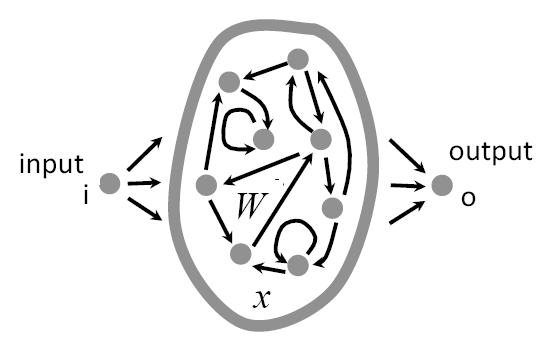
\includegraphics[width=0.8\textwidth]{img/recurrent-network}
  \caption{A General recurrent architecture maps a vectorial input sequence ${\bf i}(t)$ onto an output ${\bf o}(t)$, 
    via an internal state ${\bf x}(t)$ of hidden units. It is parameterized by a recurrent parameter matrix ${\bf W}$. 
    The dynamics is defined by the network recurrent equations.}
  \label{recurrent-network}
\end{figure}

As schematized in figure~\ref{recurrent-network}, we consider a recurrent network 
\eqline{x_n(t) = \Phi_{nt}\left(\cdots, x_{n'}(t'), \cdots, i_{m}(s), \cdots\right)}
with nodes of the form:
\begin{equation}\label{eq-recurrent}
\begin{array}{rcl} 
x_n(t) &=& \Phi_{n0t}\left(\cdots, x_{n'}(t'), \cdots, i_{m}(s), \cdots\right) \\ 
          &+& \sum_{d = 1}^{D_{n}} W_{nd} \, \Phi_{ndt}\left(\cdots, x_{n'}(t'), \cdots, i_{m}(s), \cdots\right) \\
o_n(t) &=& x_n(t), n < N_0 \\
 \end{array}
\end{equation} 
i.e., defined as a linear combination of some kernel $\Phi_{ndt}()$.
We show in Appendix~\ref{generality} that this a very general form
(e.g., including when considering the adjustment of unit parameters
that are not connection weights).

More precisely, equation~(\ref{eq-recurrent}) elements define:
 \\  -  $N$ nodes of value $x_{n}(t)$ indexed by $n \in \{0, N\{$, 
 \\  \hphantom{0.5cm} -  with a maximal state recurrent causal range of $R$ and with either,  
 \\  \hphantom{0.8cm} -  $t - R \leq t' < t$ (i.e., taking into account previous value up to $R$ time-steps in the past) or
 \\  \hphantom{0.8cm} -  $t' = t$ and $n < n'$ (i.e., taking into account present value, of subsequent nodes, in a causal way).
 \\  \hphantom{0.5cm} - while $N_0 \leq N$ of these nodes are output;
 \\  - $M$ input $i_{m}(s)$ indexed by $m \in \{0, M\{$, $t - S \leq  s < t$, 
 \\  - $1 + D_{n}$ predefined kernels $\Phi_{ndt}\left(\right)$ for each node, defining the network structure;
 \\  - $\sum_n D_n$ static adjustable weights $W_{nd}$, defining the network parameter.

\vphantom{1cm}

Considering equation~(\ref{eq-recurrent}) we notice that : \begin{itemize}

\item The distinction between output or hidden node is simply based on the fact that we can (or not) observe the $o_n(t)$ node value. Here, without loss of generality, output nodes are the $N_0 \leq N$ first ones.

\item Though, in order to keep compact notations, we mixed node with either 
 \\ \hphantom{0.2cm} - {\em unit firmware} parameter-less function, i.e. with $\Phi_{n0t}()$, or
 \\ \hphantom{0.2cm} - {\em unit learnware} linear combination of elementary kernels, i.e. with $\sum_{d} W_{nd} \, \Phi_{ndt}()$,
\\ in all examples these two kinds of node will be separated. This constraint is not mandatory, but will help clarifying the role of each node.

\item A given state value depends either on previous time values ($t - R \leq t' < t$) or subsequent indexed nodes ($t' = t$ and $n < n'$), yielding a causal dependency in each case.

\item By design choice, as made explicit in appendix~\ref{generality} for all examples, $0 \leq \partial_{x_{n'}(t')} \Phi_{ndt}() \leq 1$ (non-decreasing contractive non-linearity), is verified. This constraint is not mandatory, but will help at the numerical conditioning level.

\item We further assume, just for the sake of simplicity\footnote{It is an easy task to introduce non-zero initial conditions as additional network parameter to learn, or consider then as a transient additional random input.}, that initial conditions are equal to zero, i.e., ${\bf x}(t) = 0, t < 0$ and ${\bf i}(s) = 0, s < 0$. 

\item We also assume that the dynamic is regular enough\footnote{Here, we assume that input and output are bounded, while the system is regular enough for the subsequent estimation to be numerically stable. Chaotic behaviors likely require very different numerical methods (taking explicitly the exponential dependency on previous value variations into account) \cite{cessac_view_2010}. In practice, not only contracting systems can be considered, as soon as the observation times are not too large with respect to cumulative rounding errors. As far as computing capabilities are considered, systems at the edge of chaos (but not chaotic) seem to be interesting to consider \cite{bertschinger-natschlager:04,Legenstein:2007}, which fits with the present requirement.} for weight estimation to be numerically stable.

\end{itemize}

The key point here, is that some state variables ${\bf x}_n$ are additional intermediate internal variables in order the weight estimation to be a simple linear problem as a function of these additional variables (and at the cost of higher dimensional problem).

The claim of this paper is that this choice of notation has two main consequences developed in the next sections: \begin{enumerate}
\item All known computational networks architecture can be specified that way. This is made explicit in appendix~\ref{generality}.
\item The weight estimation problem writes in a quite simple way, with this reformulation. This is discussed now.
\end{enumerate}

\section*{Formalizing the recurrent weight estimation}

We implement the recurrent weight estimation as a variational problem, i.e. define weights as: \begin{equation}\label{eq-criterion} {\bf W} = \mbox{arg min}_{{\bf W} , {\bf x}} \; {\cal L}({\bf W} , {\bf x}) ,\end{equation}
writing:
\[ \begin{array}{clll} \multicolumn{3}{l}{{\cal L}({\bf W} , {\bf x}) \deq} \\
& \sum_{nt} & \rho_{nt}(x_n(t)) & \mbox{\small desired values} \\
-& \sum_{nt} & \varepsilon_{nt} \, (\hat{x}_n(t) - x_n(t)) & \mbox{\small network dynamic constraint} \\
+& {\cal R}({\bf W}) & & \mbox{\small regularization} \\
\end{array} \]
and represent the dynamic network recurrent equation via the notation of equation~(\ref{eq-recurrent}):
 \[ \left\{ \begin{array}{rcl}
\hat{x}_n(t) &\deq& \Phi_{n0t}\left(\cdots, x_{n'}(t'), \cdots, i_{m}(s), \cdots\right) \\
 &+& \sum_{d = 1}^{D_{n}} W_{nd} \, \Phi_{ndt}\left(\cdots, x_{n'}(t'), \cdots, i_{m}(s), \cdots\right)
\end{array} \right. \]
while $\varepsilon_{nt}$ are Lagrange multipliers.

Here $\rho_{nt}()$ is a cost-function (acting both as supervised and unsupervised variational term, as detailed in the next section) and ${\cal R}({\bf W})$ a regularization term. The cost function includes both the term attached to the data, i.e., the fact that output values have a desired values, and regularization. These ingredients are going to be used in the sequel to control approximate desired output, yield sparse estimation, reduce artifact influence, obtain activity orthogonality, etc.

Stating the estimation this way, leads us to a simplified form of the Pontryagin's minimum principle, well-known in control theory \cite{astrom:83}. The effective related solution is derived from the normal equations of the proposed criterion.

This formulation is not new and has been formalized, by, e.g. \cite{cun_theoretical_1988}. Here we restate it at a higher level of generality, with two new aspects: (i) making explicit the role of the Lagrange multiplier (also called adjoint state in this context) for hidden units and (ii) embedding this mechanism in more general learning schemes.

Applying standard derivations, the criterion gradient writes:
\[ \begin{array}{rcll}
\nabla_{\varepsilon_{nt}} \, {\cal L} &=& \hat{x}_n(t) - x_n(t) \\
&&\\
\nabla_{x_{n'}(t')} \, {\cal L} &=&  
-\varepsilon_{n't'} + \rho'_{n't'} + \sum_{nt, \begin{array}{c} t' < t \leq t' + R \\ or\; t' = t, n < n'\end{array}} \beta_{n't'}^{nt} \, \varepsilon_{nt} \\
&&\\
\nabla_{W_{nd}} \, {\cal L}  &=& \sum_{n'', W_{n''d} = W_{nd}} \sum_t \phi_{n''dt} \, \varepsilon_{n''t} + \nabla_{W_{nd}} \, {\cal R} \\
\end{array} \]
writing : {\small \[ \left\{ \begin{array}{rclcl}
\varepsilon_{nt} &\deq&  \varepsilon_{nt} + \rho'_{nt}\\
&\\
\rho'_{nt} &\deq&\rho'_{nt} \, (\hat{x}_n(t)) \\
&\\
\phi_{ndt} &\deq& \Phi_{ndt}\left(\cdots, x_{n'}(t'), \cdots, i_{m}(s), \cdots\right) &=& \nabla_{W_{nd}} \hat{x}_n(t)\\
&\\
\beta_{n't'}^{nt} &\deq& \frac{\partial \phi_{n0t}}{\partial x_{n'}(t')} + \sum_{d = 1}^{D_{n}} W_{nd} \, \frac{\partial \phi_{ndt}}{\partial x_{n'}(t')} &=& \nabla_{x_{n'}(t')} \hat{x}_n(t) \\
&\\
\end{array} \right. \]}

The sum $\sum_{nt, \begin{array}{c} t' < t \leq t' + R \;or\; t' = t, n < n'\end{array}}$ encounters for previous values and subsequent node values. This sum includes terms with $\beta_{n't'}^{nt} \neq 0$, i.e. terms for which there is a recurrent connection from the node of index $n$ at time $t$ onto the node of index $n'$ at time $t'$. We simply write $\sum_{nt}$ in the sequel, without any risk of ambiguity.

The sum $\sum_{n'', W_{n''d} = W_{nd}}$ encounters for weight sharing, i.e., the fact that weights from different units may be constrained to have the same value. We will simply write $\sum_{n''}$ in the sequel, without any risk of ambiguity.

Let us now review and discuss how we can implement such a minimization.

\subsection*{The minimization steps}

\subsubsection*{Forward simulation}

The equation $\nabla_{\varepsilon_{nt}} \, {\cal L} = 0$ yields $x_n(t) = \hat{x}_n(t)$, which simply corresponds to equation~(\ref{eq-recurrent}). Since $\hat{x}_n(t)$ depends on previous values at time $t' < t$, it provides a closed-form formula to evaluate $x_n(t)$ from the beginning to the end. This simply corresponds to the fact that the dynamic is simulated. This step depends on the weights $W_{nd}$ but not on the Lagrange multipliers $\varepsilon_{nt}$. At the end of the step the equality $\nabla_{\varepsilon_{nt}} \, {\cal L} = 0$ is obtained, and the criterion value itself does not depends on $\varepsilon$ since the constraints are verified. As a consequence, the criterion value ${\cal L}$ can be calculated during this step.

The forward simulation complexity corresponds to the network simulation and is of order $O(N D T)$ with a memory resources of $O(N T)$ since we must buffer the calculated output,  for subsequent calculations.

\subsubsection*{Backward tuning}

The equation $\nabla_{x_{n'}(t')} \, {\cal L}  = 0$ also provides a closed-form formula to evaluate $\varepsilon_{n't'}$ as a linear function of subsequent values $\varepsilon_{nt}, t > t'$, so that the calculation is to be done from the last time $t = T-1$ backward to the first time $t = 0$.

This is the key feature of such a variational approach, allowing backward tuning, i.e., take into account the fact that adjusting the system parameters for a node $n$ at time $t$ is interdependent with the state of subsequent computations.

If $\beta_{n't'}^{nt} = 0$, there is no dependency of ${x}_n(t)$ on ${x}_{n'}(t')$, and in the absence of recurrent connection $\varepsilon_{n't'} = 0$ and $\varepsilon_{n't'}$ only depends on the state cost function $\rho'_{nt}$.

As mentioned by \cite{cun_theoretical_1988}, $\beta_{n't'}^{nt}$ is nothing more than the first order approximation of the backward dynamics, technically the product of the weight matrix with the system Jacobian.

This backward computation is local to a given unit in the sense that only efferent units (i.e., units this unit is connected to) are involved in the computation of the related Lagrange parameter. This step depends on both weights and output values, and the equality $\nabla_{\varepsilon_{nt}} \, {\cal L} = 0$ is obtained at the end.

The backward tuning step has the same order of magnitude in terms of calculation $O(N D T)$  and memory resources of $O(N T)$ (in fact of $O(N R)$, because the obtained result may be immediately re-used to compute the weight adjustment gradient or 2nd order system). 

\paragraph{\em Parameter interpretation.}

We obtain, after some algebra:
\\\centerline{$\varepsilon_{n't'} = \rho'_{nt} + \sum_{nt} \beta_{n't'}^{nt} \, \varepsilon_{nt} = \sum_{nt} B_{n't'}^{nt} \, \rho'_{nt}$}\\ with finite summations and for some quantities $B_{n't'}^{nt}$ (not made explicit here) which are unary coefficient polynomial in $\beta_{n't'}^{nt}$. This made explicit the fact $\varepsilon_{n't'}$ is a linear function of subsequent errors, i.e., a backward tuning error.

If the unit has no recurrent connection, i.e. is a not a function of other units, then $\varepsilon_{n't'} = \rho'_{nt}$ is simply related to the cost function. In the least-square case (i.e. if $\rho_{nt} = \frac{1}{2} \, (x_{nt} - \bar{o}_{nt})^2$), then $\rho'_{nt} = x_{nt} - \bar{o}_{nt}$ is the output error.

It must be noted, that this method is quite different from back-propagation-though-time recurrent network estimation or other standard alternatives. If the calculation may be recognized as a kind of back-propagation, it is mathematically different.

\paragraph{\em Numerical stability.}

However, as reviewed in e.g., \cite{Hochreiter:1997} this back-propagation of tuning error, will suffer form the same curse than back-propagation of gradient: Either error explosion (if $|\beta_{n't'}^{nt}| > 1$), or error vanishing (if $|\beta_{n't'}^{nt}| < 1$). In our case, since all kernels are contracting we have the bound, writing $\beta_{max} \deq \max_{nt} |\beta_{n't'}^{nt}|$ :
\\\centerline{$0 \leq \left|\beta_{n't'}^{nt}\right| \leq \beta_{max} \leq 1 + \sum_d |W_{nd}|$}\\
without any thinner inequality in the general case. Based on this remark, the key idea of LSTM \cite{Hochreiter:1997} is to consider memory carousel as reviewed in the previous section to guaranty $\left|\beta_{n't'}^{nt}\right| \simeq 1$ and thus a stable back-propagation for at least some recurrent link. In our framework this means that it is the responsibility of the designer of the network architecture to consider nodes with such property.

Here, we are going to introduce another heuristic and {\em bias} the backward error in order to avoid both error explosion and vanishing. To this end, we define:
\begin{equation} \label{kappa}
\kappa_{n't'} = \rho'_{nt} + g_{\epsilon}\left(\sum_{nt} \beta_{n't'}^{nt} \, \kappa_{nt}, \beta_{max}\right),
\end{equation} considering a function $g_{\epsilon}(u, \beta_{max})$ yielding both amplification of small errors and saturation of larger error, while at the algorithm convergence we need to have $g(u) = u$ in order to yield an unbiased estimation. Here is a continuation parameter, with $\epsilon = 1$ at the minimization start, while $\epsilon \rightarrow 0$ with algorithm convergence. It is adjusted by the minimization algorithm, which looks for a convergence at $\epsilon = 1$ and then decreases $\epsilon$ while tracking the minimum during $\epsilon$ decrease.

A simple choice is to consider an exponential saturation. Taking into account the previous requirements, for $0 < \epsilon < 1$, writes:
\\\centerline{$g_{\epsilon}(u, \beta_{max}) \deq  sg(u) \, \left(1 + \beta_{max}\,\frac{1-\epsilon}{\epsilon}\right) \, \left(1 - e^{-\frac{\epsilon}{\beta_{max}} \, |u|}\right)$}\\
and it is obvious to verify that:
\\\centerline{$\begin{array}{rcll} g_{\epsilon}(u, \beta_{max}) 
 &=& u + O(\epsilon) & \mbox{convergence to identity when $\epsilon \rightarrow 0$} \\
 &=& \frac{u}{\beta_{max}} + O(u^2) + O(1 - \epsilon) & \mbox{amplification around $\epsilon = 1$} \\
 &<& \frac{1}{\epsilon} & \mbox{saturation for non negligible $\epsilon$} \\
 &\leq& \left((1 - \epsilon) + \frac{\epsilon}{\beta_{max}}\right) \, u & \mbox{concave profile} \\
\end{array}$}\\
The convergence to identify is uniform for bounded values of $u$ and the amplification leads to $\left|\frac{\partial g(\dot)}{\partial \kappa_{nt}}\right| \leq 1$ but as closed as possible to 1, avoiding any propagation explosion, with at least some non negligible backward tuning. With the decrease of $\epsilon$ we may and must relax this constraint, but can reasonably expect the backward tuning error to decrease with the criterion convergence, the related quantities to remain bounded.

\paragraph{\em Real-time aspects.}

Such a formulation is definitely not ``real-time'', since we ``go back in time''. It is however, the only solution for hidden layers to be tuned, since the output is a function of hidden activity in the past. 

However, in a real-time paradigm, it must be noted that each computation is also local in {\em time}: It only depends on values in a ``near future'' within a time range equal to the system time range. In other words, at a given time we obtain the value with a lag equal to system time-range. It is an interesting perspective of this work to explore if, in a rather stationary context, it may provide numerically relevant values for on-the-fly backward tuning.

\subsubsection*{The 1st order unit weight adjustment}

The calculation of $\nabla_{W_{nd}}\, {\cal L} $ yields a Hebbian weight adaptation rule (as the sum of products between an output unit error term $\varepsilon_{nt}$ (combining the supervised error and the backward tuning multiplier) and an input quantity $\phi_{ndt}$. This rule applies to both output unit of index $n < N_0$ with a desired output and hidden units of index $N_0 \leq n$ that indirectly adapt their behavior to optimize the output, via the backward tuning values. The gradient calculation is local to a given unit and average over time, through another $O(NDT)$ computation.

This leads to a local 1st order adjustment of the weights, i.e. it provides the direction for the weight variation, not its magnitude.

To numerically adjust this magnitude we have to perform a 1D minimization, i.e., $\mbox{min}_{\upsilon^k} \; {\cal L}({\bf W}(\upsilon^k) , \tilde{\bf x})$, with:
\\\centerline{$W_{nd}(\upsilon^k) = \tilde{W}_{nd} - \upsilon^k \, \nabla_{\tilde{W}_{nd}} \, {\cal L}, \mbox{ with } 0 < \upsilon^k$} \\
where $\tilde{\bf W}$ and $\tilde{\bf x}$ correspond to the previous estimation of the weights and activity. This minimization can be local to each unit. The key point is that we do not know any reasonable upper-bound for $\upsilon^k$. As a consequence standard golden section search or Brent-Dekker methods do not directly apply, and we have to numerically find such an upper-bound first, and it appeared that which requires additional calculation steps. It is also known that it is inefficient to precisely find the minimum since the gradient value varies with $W_{nd}$ so that the result is anyway biased. Taking all this into account, we obtain the 1st order unit weight adjustment heuristic:\begin{quotation}{\small 
\noindent -0- Starts with the last known value of $\upsilon^k$ or very small value (here $10^{-6}$).
\\-1- Computes ${\cal L}(W_{nd}(\upsilon^k))$.
\\\hspace{0.5cm} -2.1- If it decreases, register this better value, and set $\upsilon^k = 2\, \upsilon^k$ for the next step, 
\\\hspace{0.5cm} -2.2- else set $\upsilon^k = \upsilon^k / 3$.
\\-3- Repeat -1- unless steps -2.2- leads to a negligible value of $\upsilon^k$.
}\end{quotation}
Each step requires a simulation to compute ${\cal L}$.

It is easy to verify that this tiny heuristic converges and provides an approximation of the minimum. It also provides an upper-bound for usual minimum search methods, but it has be numerically observed, at the global minimization level, that adding such search methods is useless (it slows-down the minimization with only a negligible gain in precision, if any).

As far as backward tuning stability is concerned the value of $\varepsilon_{nt}$ is replaced by its approximation $\kappa_{nt}$.

The 1st order unit weight adjustment could either be done globally at the whole node set level, or locally for each unit, the criterion itself being decomposable on each unit. In this latter case, the global convergence is guaranty only with infinitesimal gradient steps.

\subsubsection*{The 2nd order unit weight adjustment}

Due to the simplicity of the approach, we can write a 2nd order weight adjustment:
\[
\nabla_{W_{nd}} \, {\cal L} = 0 \Rightarrow \sum_{n''} b_{n'',\,d} = \sum_{n''} \sum_{d'=1}^{D_{n}} A_{n'',\,d\;d'} \, W_{nd'}
\] writing, for some $\kappa_{nt}$: \[ \left\{ \begin{array}{rcl}
b_{n,\,d} &\deq& \sum_t \phi_{ndt} \, \left( \varepsilon_{nt}  + \kappa_{nt} \, \left(\hat{x}_n(t) - \phi_{n0t} \right) \right)  + \nabla_{W_{nd}} \, {\cal R}(\tilde{\bf W}),  \\
&\\
A_{n,\,d\;d'} &\deq& \sum_t \kappa_{nt} \, \phi_{ndt} \, \phi_{nd't}.  \\
\end{array} \right. \]
This allows to obtain a new weight value $\tilde{\bf W}$ solving a linear system of equation for each unit, where $\hat{x}_n(t)$ is calculated taking the previous or initial weight value $\hat{\bf W}$ into account.

Here indeed, the value of $\kappa_{nt}$ corresponds to the backward tuning stability proposed heuristic.

The chosen form is related to the 2nd order Hessian of the criterion\footnote{
\label{criterion-hessian} The criterion Hessian, omitting the regularization term, writes: \\ \centerline{$\left.\begin{array}{rcl}
\nabla_{W_{nd} W_{n'd'}} \, {\cal L} &=& \delta_{n=n'} \, \sum_t \, \rho''_{nt} \, \phi_{ndt} \, \phi_{nd't} 
\end{array}\right.$}\\
\\ Here the notation $\delta_{\cal P}$ stands for $1$ is the property ${\cal P}$ is true and $0$ otherwise.
\\ A step further, for the sake of completeness we also make explicit (writing $\beta_{nt}^{nt} \deq -1$ ):
\\ \centerline{$\left\{\begin{array}{rcl}
\nabla_{\varepsilon_{nt} \varepsilon_{n't'}} \, {\cal L} &=& 0 \\
&&\\
\nabla_{x_{n'}(t') \varepsilon_{nt}} \, {\cal L} &=& \beta_{n't'}^{nt} \\
&&\\
\nabla_{W_{nd} \varepsilon_{n't'}} \, {\cal L} &=& \delta_{n=n'} \, \phi_{ndt'} \\
&&\\
\nabla_{x_{n'}(t') x_{n''}(t'')} \, {\cal L} &=&  \sum_{nt} \rho''_{nt} \, \beta_{n't'}^{nt} \, \beta_{n''t''}^{nt}
 \\&+& \left[ \frac{\partial^2 \phi_{n0t}}{\partial x_{n'}(t') x_{n''}(t'')} + \sum_{d = 1}^{D_{n}} W_{nd} \, \frac{\partial^2 \phi_{ndt}}{\partial x_{n'}(t') x_{n''}(t'')} \right] \, \varepsilon_{nt}, \\
&&\\
\nabla_{W_{nd} x_{n'}(t')} \, {\cal L} &=&  \sum_{t} \rho''_{nt} \, \beta_{n't'}^{nt} \, \phi_{ndt}
 + \frac{\partial \phi_{ndt}}{\partial x_{n'}(t')} \, \varepsilon_{nt}, \\
\end{array}\right.$.}} and generalizes the readout least-square estimation of weights\footnote{
For a simple least-square criterion of the form:
\\ \centerline{${\cal L} = \sum_{nt} \frac{\kappa_{nt}}{2} \, (\hat{x}_n(t) - \bar{o}_n(t))^2$} \\
where $\kappa_{nt} \in \{0, 1\}$ depending on the fact that the desired output $\bar{o}_n(t)$ is defined or not, it is straight-forward to verify the proposed 2nd order weight adjustment holds, and reduces to an exact linear system of equation, in the absence of recurrent links of the given unit, since $\phi_{ndt}$ is only function of the input. Otherwise, we only $\phi_{ndt}$ is also a function of both the network unknown output and hidden node values. For output node value the $\bar{o}_n(t)$ desired value could be enforced, limiting recurrent perturbation and yielding $\phi_{ndt}$ values closed to the ideal value, which is interesting in reverse-engineering estimation, i.e. when an exact solution is expected \cite{rostro-gonzalez-cessac-etal:10}, whereas a bias in the estimation is otherwise introduced.} in a neural network.

The weight adjustment is local to each unit, providing a true distributed mechanism. This corresponds to a 2nd order minimization scheme. Each step requires $O(N (D T + D^3)$ operation, solving a linear system of equations. The implemented method is a Cholesky decomposition with a fallback onto a singular-value-decomposition if the ${\bf A}_n$ is not strictly positive.

Taking all this into account, we obtain the following 2nd order unit weight adjustment heuristic:\begin{quotation}{\small 
\noindent -0- Calculates $\tilde{\bf W}$ and starts with $\upsilon^k = 1$.
\\-1- Computes ${\cal L}(\upsilon^k \tilde{\bf W} + (1 - \upsilon^k) \, \hat{\bf W})$.
\\\hspace{0.5cm} -2.1- If it decreases, register this better value, 
\\\hspace{0.5cm} -2.2- else set $\upsilon^k = \upsilon^k / 2$.
\\-3- Repeat -1- unless steps -2.2- leads to a negligible value of $\upsilon^k$.
}\end{quotation}
In words we look for a weight value between both previous and new values that decreases the criterion. Each step requires a simulation to compute ${\cal L}$.

\subsubsection*{The complete weight adjustment}

Collecting previous steps the final iterative weight adjustment writes\begin{quotation}{\small 
\noindent -1- Performs a forward simulation and a backward tuning, calculating the 1st order gradient and 2nd order elementsduring the backward estimation.
\\\hspace{0.5cm} -2.a- Attempt to perform a 2nd order weight adjustment.
\\\hspace{0.5cm} -2.b- If it fails, attempt to perform a 1st order weight adjustment.
\\-3- Repeat -1- unless steps -2.b- fails.
}\end{quotation}
This weight adjustment has to be performed by continuation using the modified numerically stable backward tuning calculation.

The present proposal stands on the fact that we have been able to derive a local 2nd order adjustment based on renormalized backward tuning. The 1st order fall-back method could indeed have been enhanced using either the so called momentum gradient mechanism (based on a temporal averaging of the gradient values), or the partial conjoint gradient methods (taking into account several subsequent gradient directions in order to infer an approximate 2nd order mimimization method. We also propose here an alternative to 2nd order adjustment methods such as \cite{martens_learning_2016} or other methods reviewed in \cite{Goodfellow2016Deep}.


\section*{Experimentation}

In this experimental part we are going to both study the numerical stability and limit of the method and compare to existing non-trivial benchmark problems. Here, supervised learning is targeted since it is a direct way to evaluate the method efficiency and robustness. Let us remember that we do not evaluate learning performances here, only the way me can adjust recurrent network weights. We only study the estimation convergence here, not the learning properties (such as generalization, capacity, ...).

\subsection*{Software implementation}

In order to provide so called reproducible science \cite{topalidou_long_2015}, the code is implemented as a very simple, highly modular, fully documented, open source, object oriented, easily forkable, self contained, middle-ware, \href{nowhere:not-yet-on-line}{available here}. A minimal set of standard mechanisms (random number generation, histogram estimation, linear system resolution, system calls) is used. The main part of the implementation hierarchy is show in Fig.~\ref{class-hierarchy}. 

\begin{figure}[!ht]
  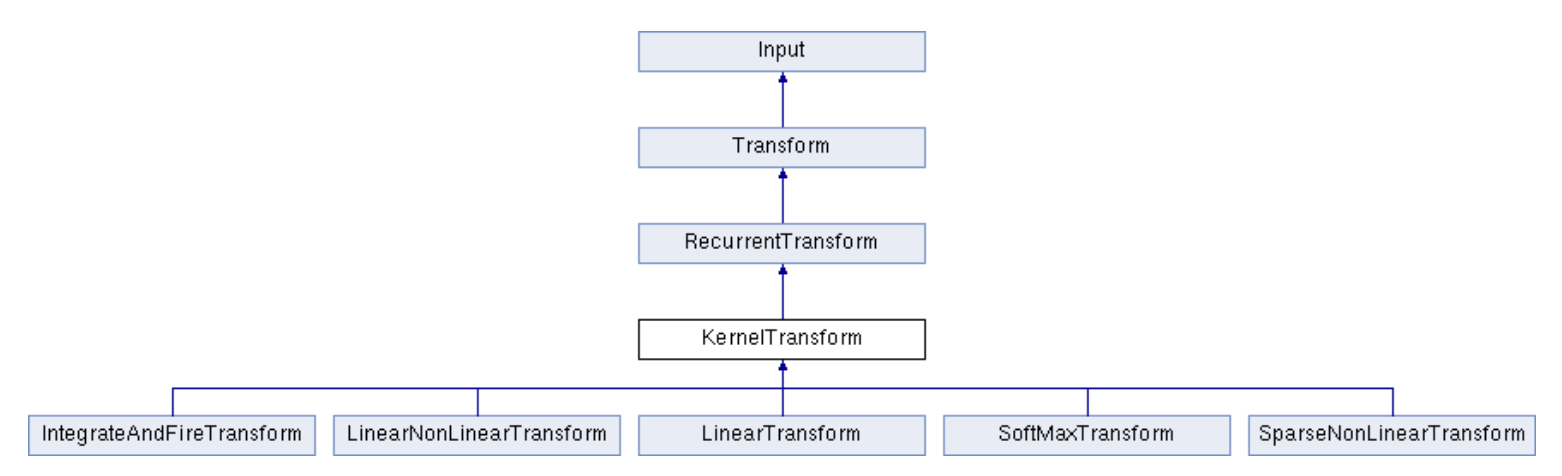
\includegraphics[width=0.8\textwidth]{img/class-hierarchy}
  \caption{A view of the class-hierarchy: A {\tt Input} simply provides a $x_n(t), n \in \{0, N\{, t \in \{0, T\{$ values, while a {\tt Transform} provides such values given another {\tt Input}, while other objects defined here derive from such an oversimple abstract class.}
  \label{class-hierarchy}
\end{figure}

For run-time performances and inter-operability with different programming languages a {\tt C/C++} implementation (with the compilation scripts) is proposed, the wrapping to other programming languages (e.g., {\tt Python}) being straightforward, using e.g. {\tt swig}. 

The first experimental verification was that it was very simple to define the main unit structures reviewed in section~\ref{generality} from {\tt KernelTransform} as claimed in the paper.

\subsection*{Numerical stability and limit of the method}

Regarding this first issue, as being in a deterministic context, we are going to rely on a reverse engineering setup: An input/output learning sequence is going to be generated by a input/output root network of $\bar{N}$ units and another learning network with random initialization is going to re-estimate a transform. This guaranty the existence of an exact solution. 

How revelant is it to use such a reverse engineering setup ? On one hand, surprisingly enough perhaps, such networks (at least deep networks \cite{Zhang2016Understanding}) behave with the same order of magnitude of performances, the input being either ``meaningful'' in the sense it represents data with a semantic or not. We thus can expect simple random input/output tests to be relevant to more specific application. On the other hand we are going to develop in the next section how several ``challenging'' tests are in fact highly dependent on the chosen architecture, with often trivial solution, as soon as the hidden architecture is well chosen.

Considering random input/output with some statistics, in most of the cases, they are several solutions (e.g. up to a permutation of the units, or some linear combination in a linear case, ...). We consider a root network of $\bar{N}$ units for a sequence of time $T$, for a $M=1$ scalar input, considering either L (for linear), LNL or AIF units, with random weights (drawn from a Gaussian distribution with $0$ mean and $\sigma \simeq 1/N$ standard deviation, which is know to guaranty a stable non-trivial dynamic). Only the unit of index $n=0$ is considered as output units, i.e., $N_0 = 1$, the $N-1$ remainder units activity being hidden to the estimation.

In this determistic case, we observe two main parameters the final precision criterion value ${\cal L}$ and the number of steps to convergence $S$. 

A step further, we also study exact solution or approximation, we are going to consider learning network with $N \leq \bar{N}$ units, i.e. networks that do not generate the exact solution. We already know that as soon as the dynamic is sufficiently rich, even small errors accumulates and the solution exponentially diverges from the exact one. In such a case the question is wether the input/output statistics also diverges. We thus have to compare the KL-divergence between the desired and obtained output given the input. The fact we chose $N_0 = 1$ makes this estimation tracktable since it is a 1D distribution. OUI MAIS JUSTE HISTOGRAMME QUID DE LA DEPENDENCE EN i(t-R) ?

\subsection*{Comparison with existing estimation problems}

Let us now discuss how our validation method compares with usual benchmark for recurrent network estimation.

\section{Conclusion}We consider another formulation of weight estimation in recurrent networks, proposing a notation for a large amount of recurrent network units that helps formulating the estimation problem. Reusing a ``good old'' control-theory principle, improved here using a backward-tuning numerical stabilization heuristic, we obtain a numerically stable and rather efficient second-order and distributed estimation, without any meta-parameter to adjust. The relation with existing technique is discussed at each step. 
The proposed method is validated using reverse engineering tasks.


\appendix
\clearpage\section{Major examples fitting this architecture.} \label{generality}

The notation of equation~(\ref{eq-recurrent}) seems to be the most general form of usual recurrent networks. Let us state this point by considering several examples of units, and make explicit how we decompose them in term of nodes.

\paragraph{Linear non-linear (LNL) units.} 

Such network unit corresponds to the most common\footnote{See also a dual form related to AIF, in the sequel, with an alternate insertion of the non-linearity.} network unit and is defined by a recurrent equation of the form:
\begin{equation}\label{lnl-network}
\begin{array}{rcl}x_n(t) &=& \gamma_n \, x_n(t-1) \\ &+& \zeta_{[a,b]}\left(\alpha_n + \sum_{n' = 0}^{N-1} W_{nn'} \, x_{n'}(t-1) + \sum_{m = 0}^{M-1} W_{nm} \, i_m(t-1)\right), \end{array}\end{equation}
\\- with either a fixed or adjustable {\em leak}\footnote{Here $\gamma = 1 - \frac{\Delta T}{\tau}$ stands for the leak of each unit, writing $\Delta T$ the sampling period, $\tau$ the continuous leak and using an basic trivial Euler discretization scheme, the $\zeta()$ profile being re-normalized accordingly.} $\gamma_n$, providing $0 < \gamma_n < 1$, and 
\\- optionally {\em intrinsic plasticity} parameterized by $\alpha_n$. 

The {\em non-linearity} often\footnote{If the model corresponds to a rate, i.e., a firing probability, we can use the logistic sigmoid, which writes $\zeta_{[0,1]}(u) = \frac{1}{1 + e^{-4 \, u}} = \frac{1 + \tanh(2 \, u)}{2}$.} writes
\eqline{\zeta_{[a,b]}(u) \deq \frac{a+b}{2} + \frac{b-a}{2} \, \tanh(\frac{2}{b-a} \, u),}
with $\zeta_{[a,b]}(-\infty) = a, \zeta_{[a,b]}(+\infty) = b, \zeta_{[a,b]}(u) = \frac{a+b}{2} + u + O(u^3)$,  while $\zeta'(u) = 1 - \tanh(\frac{2}{b-a} \, u)^2$,  $0 < \zeta'(u) \leq 1$, with $\max|\zeta'(u)| = 1$, thus contracting with a correct numerical conditioning. We mainly have $[a,b] = [0,1]$ or $[a,b] = [-1,1]$ depending on the semantic interpretation of the $x_n(t)$ variable.

Another form of non-linearity is a rectified linear unit (or ReLU), i.e.:
\eqline{\zeta_{[0,+\infty]}(u) \deq \max(0, u).}
This function is not derivable at $u = 0$. It is however very easy to consider a mollification (called ``softplus'') e.g., $\zeta_{\epsilon, [0,+\infty]}(u) \deq \epsilon \, \log\left(1 + e^{\frac{u}{\epsilon}}\right)$ which is an analytic smooth approximation which uniformly converges\footnote{Since $\forall u, |\zeta_{\epsilon, [0,+\infty]}(u) - \zeta_{[0,+\infty]}(u)| \leq \log(2) \, \epsilon$.}, i.e. $\lim_{\epsilon \rightarrow 0} \zeta_{\epsilon, [0,+\infty]}(u) = \zeta_{[0,+\infty]}(u)$. See the section on AIF units to see how to adjust, if needed, such a meta-parameter redefining it as a node parameter.

For adjustable leak we need three nodes to fit within the proposed notations:
\eqline{\begin{array}{rcl}
 x_n(t) &=& x_{n_1}(t) + \zeta_{[a,b]}\left(x_{n_2}(t)\right) \\
 x_{n_1}(t) &=& \gamma_n \, x_{n}(t-1) \\
 x_{n_2}(t) &=& \alpha_n + \sum_{n' = 0}^{N} W_{nn'} \, x_{n'}(t-1) + \sum_{m = 0}^{N} W_{nm} \, i_m(t-1) \\
\end{array}}
and it is easy to verify that this second form fits with equation~(\ref{eq-recurrent}), since:
\\- The 1st line corresponds to a parameter-less $\Phi_{n0t}\left(\right)$ kernel (unit firmware).
\\- The 2nd and 3rd lines correspond to linear combinations of elementary kernels $\Phi_{ndt}\left(\right)$ selecting another state or input variable (unit learnware).

With this example, we see that the proposed approach is to introduce two additional intermediate variables $x_{n_1}(t)$ and $x_{n_2}(t)$ related to each linear combination of weights or other parameter.

With a fixed leak (i.e., if the value $\gamma_n$ is known) the LNL unit decomposes into two nodes, a parameter less node combining $x_n(t)$ and $x_{n_1}(t)$, and the linear combination defined for $x_{n_2}(t)$.

This equation is also valid for the main auto-encoder architectures, and for convolution networks \cite{Bengio:2009,Deng:2014}, with an important additional feature : weight-sharing, i.e. the fact that several weights $W_{nd}$ are the same across different nodes. This is taken into account in this paper.

\paragraph{Long short term memory (LSTM) units.} 

Such network unit is defined by a sophisticated architecture \cite{Hochreiter:1997}, described in figure~\ref{recurrent-network}. A unit is made of the following nodes:
\begin{equation}\label{lstm-network}
\begin{array}{rcl}
\multicolumn{3}{l}{\mbox{Unit output:}} \\
x_n(t) &=& \zeta_{[0,1]}\left(y_n^{out}(t)\right) \, \zeta_{[-1,1]}\left(s_n(t)\right) \\
\multicolumn{3}{l}{\mbox{Unit state:}} \\
s_n(t) &=& \zeta_{[0,1]}\left(y_n^{forget}(t)\right) \, s_n(t-1) + 
          \zeta_{[0,1]}\left(y_n^{in}(t)\right) \, \zeta_{[-1,1]}\left(g_n(t)\right) \\
\multicolumn{3}{l}{\mbox{Unit gate:}} \\
g_n(t) &=& \sum_{n'} W^g_{nn'} \, x_{n'}(t-1) + \sum_{m} W^g_{nm} \, i_m(t-1) \\
\multicolumn{3}{l}{\mbox{Output modulation:}} \\
y_n^{out}(t) &=& W^o_n \, s_n(t-1) + \sum_{n'} W^o_{nn'} \, y_{n'}^c(t-1) + \sum_{m} W^o_{nm} \, i_m(t-1) \\
\multicolumn{3}{l}{\mbox{Forgetting modulation:}} \\
y_n^{forget}(t) &=& W^f_n \, s_n(t-1) + \sum_{n'} W^f_{nn'} \, y_{n'}^c(t-1) + \sum_{m} W^f_{nm} \, i_m(t-1) \\
\multicolumn{3}{l}{\mbox{Memorizing modulation:}} \\
y_n^{in}(t) &=& W^i_n \, s_n(t-1) + \sum_{n'} W^i_{nn'} \, y_{n'}^c(t-1) + \sum_{m} W^i_{nm} \, i_m(t-1)  \\
\end{array}\end{equation}

The first two nodes are parameter-less additive and/or multiplicative combination of non-linear functions of the reminding four nodes, which are themselves linear combination of the incoming signal gate and the input, forgetting and output modulatory signals. 

The present notation corresponds to the most general form (e.g., with peephole connections \cite{Gers:2003}) of LSTM, while several variants exist. A rather closed mechanism is named gate recurrent unit \cite{Cho-2014}, and is based on the same basic ideas of modulatory combination, but with a simpler architecture. We do not make explicit the equations for all variants of LSTM here, just notice that they correspond to some of the very best solutions for high performance recurrent network computation \cite{Schmidhuber:2015}.

\begin{figure}[!ht]
  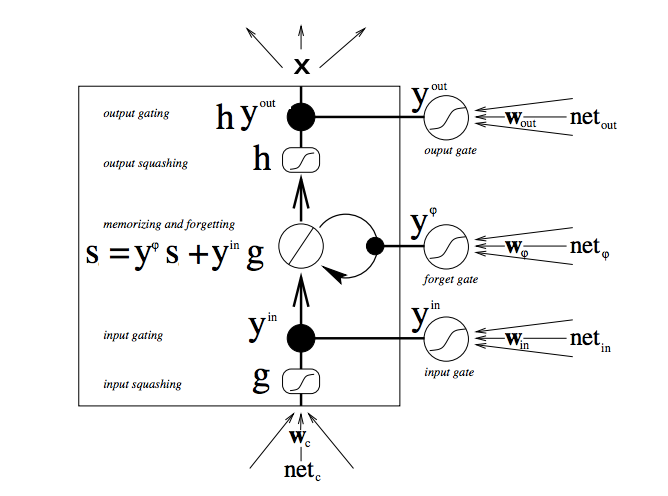
\includegraphics[width=0.8\textwidth]{img/lstm-unit}
  \caption{A LSTM unit has three processing stages for bottom to top: The (i) gate $g$ corresponds to as standard LNL unit that (ii) feeds an internal state memory $s$ which value is also driven by a forget (or remember) signal allowing to maintain the previous value, before (iii) the output connected value $x$ diffuse (or not) the result in the network. The LSTM mechanism is thus based on three ingredients, (a) the use of modulatory connection (i.e., with a multiplication by a number between 0 and 1 in order to control the signal gain), (b) a memory ``carrousel'' (i.e., an equation that could be of the form $s_n(t) = s_n(t-1)$ in order to maintain a signal, during a long short-term delay), and (c) the use of several modulatory signals. From \cite{Hochreiter:1997}.}
  \label{lstm-unit}
\end{figure}

However, in our context, instead of reusing such a complex unit as it, the design choice is to consider the non standard nodes (i.e., unit output and unit state) as modular nodes that could be combined with NLN at different level of complexity, depending on the task. At the implementation level we are not going to provide LSTM units as black boxes but an object-oriented framework allowing to adjust the network architecture to the dedicated task.

A key-point is that LSTM have, by construction, a real virtue regarding weight adjustment since back-propagation curses (vanishing or explosion) is avoided \cite{Schmidhuber:2015}. A strong claim of this paper is that we can efficiently adjust the recurrent network weights even if we do not use (or only use) LSTM but simpler units also.

\paragraph{Strongly-Typed Recurrent Neural units.} 

This other formalism \cite{Balduzzi:2016} carefully considers the signal type in the sense of parameters of different physical origins (e.g., Volts and meter), that cannot be simply mixed. This approach allows unary and binary functions on vectorial values of the same type, transformation from one orthogonal basis to another (thus using orthogonal matrices only) and component-wise product (i.e., modulatory combination). The authors show that strongly-typed gradients better behaved and that, despite being more constrained, strongly-typed architectures achieve lower training and comparable
generalization error to classical architectures. Considering a strongly-typed LNL unit, following \cite{Balduzzi:2016} and translating in the present notation, at the same degree of generality of LNL networks, we obtain:
\begin{equation}\label{st-lnl-network}\begin{array}{rcll}
  x_n(t) &=& \zeta_{[0,1]}\left(f_n(t)\right) \, x_n(t-1) + \left(1 - \zeta_{[0,1]}\left(f_n(t)\right)\right) \, z_n(t) \\
  f_n(t) &=& \alpha_n + \gamma_n \,  x_n(t-1) \\
  z_n(t) &=& \sum_{n' = 0}^{N} W'_{nn'} \, x_{n'}(t-1) + \sum_{m = 0}^{N} W'_{nm} \, i_m(t-1) \\
\end{array}\end{equation}
The first line is the firmware combination of the unit forgetting mechanism, this value being defined in the 2nd line, while the 3rd line performs the linear combination of other network values.
It is an interesting alternative to usual approach, embedable in our notation.

\paragraph{Approximation of {\em leaky integrate and fire} (AIF), current-driven, spiking-neuron unit.}

Let us also discuss how to cope with spiking networks (see \cite{cessac-paugam-moisy-etal:10} for a general discussion on such network computational power and limit).
 Following \cite{cessac_discrete_2008} (with a tiny change of notation), we consider without loss of generality a discretized form, which writes: \begin{equation}\label{lif-network} \begin{array}{rcl}x_n(t) &=& \gamma_n \, \left(1 - \Upsilon_\epsilon\left(x_n(t-1)\right)\right) \,x_n(t-1) \\ &+& \sum_{n' = 0}^{N} W_{nn'} \, \Upsilon_\epsilon\left(x_{n'}(t-1)\right) + \sum_{m = 0}^{N} W_{nm} \, i_m(t-1), \end{array}\end{equation} 
where the unit value is over or below the spiking threshold $\theta = 1/2$ (thus spiking or not), while the reset value is $0$.

Here, as inspired from \cite{cessac_using_2012}, we propose to use $\Upsilon_\epsilon(v) \deq \zeta_{[0,1]}\left(\frac{v-1/2}{\epsilon}\right)$, as a mollification of the threshold function\footnote{Obviously, $\lim_{\epsilon \rightarrow 0, v \neq 0} \Upsilon_\epsilon(v) = \Upsilon(v)$, while $\Upsilon'_\epsilon(0) = 1/\epsilon$ and $\int_v |\Upsilon_\epsilon(v) - \Upsilon(v)| = \log(2)/2 \, \epsilon$. Here the convergence can not be uniform (since a continuous function converges towards a step function), more precisely $\sup_v |\Upsilon_\epsilon(v) - \Upsilon(v)| = 1/2$ (around $v\simeq 1/2$). 
}: 
\eqline{\Upsilon(v) \deq \left\{\begin{array}{cl} 0 & v < 1/2 \\ 1/2 & v = 1/2 \\ 1 & 1/2 < v \\ \end{array}\right..}
To avoid spurious effects when adjusting the weights, we have to find out the best minimal $\epsilon$ value for each unit.

As far as the unit architecture is concerned, it is a simple variant of LNL unit, with different kernel function, and different positioning of the non-linearity. The key point is that this so called BMS formulation fits with the present approach:
\eqline{\begin{array}{rcl}
 x_n(t) &=& \gamma_n \, \left[(1-\zeta_{[0,1]}(x_{n_1}(t))) \, x_n(t-1)\right] \\ 
  &+& \alpha_n + \sum_{n' = 0}^{N} W_{nn'} \, \zeta_{[0,1]}\left(x_{n'_1}(t-1)\right) + 
      \sum_{m = 0}^{N} W_{nm} \, i_m(t-1) \\
 x_{n_1}(t) &=& \frac{1}{\epsilon} \, \left[x_n(t-1) - \frac{1}{2} \right] \\
\end{array}}
Here $\omega\deq\frac{1}{\epsilon}$ is now a parameter to estimate, in order each unit to be a suitable approximation of a spiking activity. This differs from \cite{cessac_using_2012} where sharpness was considered as a meta-parameter: Here it is a parameter learned on the data. In both cases, we need ${\epsilon \rightarrow 0}$, which means that the transformation is very sharp, limiting the numerical stability. This is going to be investigated at the numerical level.

The use of such units is very interesting in practice and we review in appendix~\ref{closedforms} how they can be used to propose trivial solutions to rather complex tasks.

\paragraph{Softmax and exponential probability units.} 

When considering exponential distribution of probability on one hand, or softmax\footnote{
The relation with a max operator comes from the fact that:
\eqline{x_n(t) \deq \frac{e^{\frac{z_n(t)}{\epsilon}}}{\sum_n e^{\frac{z_n(t)}{\epsilon}}} \Rightarrow \lim_{\epsilon \rightarrow 0} \sum_n x_n(t) \, z_n(t) = \max_n \left( z_n(t)\right).}
In words the softmax weighted sum of values approximates these values maximum.} computation on the other hand, one comes to the same equation\footnote{See, e.g., \url{https://en.wikipedia.org/wiki/Softmax\_function}.} which writes: \begin{equation}\label{exp-network}\begin{array}{rcl}
x_n(t) &=& \frac{e^{z_n(t)}}{\sum_n e^{z_n(t)}} = \exp\left(z_n(t) - \log(\sum_n \exp\left(z_n(t)\right)\right) \\
z_n(t) &=& \alpha_n + \sum_{n' = 0}^{N} W'_{nn'} \, x_{n'}(t-1) + \sum_{m = 0}^{N} W_{nm} \, i_m(t-1) \\
\end{array} \end{equation} with $\sum_n x_n(t) = 1$ in relation with the so-called partition function $Z(t) = \sum_n \exp\left(z_n(t)\right) > 0$. 

This kind of unit, in addition to NLN units, or LSTM units form the basic components of deep-learning architectures \cite{Bengio:2009,Deng:2014}.

The 1st line is a firmware global equation\footnote{It is worthwhile mentioning that:
\eqline{\partial_{z_{n'}(t)} o_n(t) = o_n(t) \, \left(\delta_{n=n'} - o_{n'}(t)\right) \in [0,1], \delta_{n=n'} = \left\{\begin{array}{cl} 1 & n = n' \\ 0 & \mbox{otherwise} \end{array}\right.,}
thus numerically well defined, with no singularity, the transformation being contracting, i.e., $\left|\partial_{{\bf z}} {\bf o}\right| \leq 1$, with $\max|\partial_{{\bf z}} {\bf o}|=1$.} which is a function of all units value of the same layer.

We encounter such a construction in restricted Boltzmann machine (RBM) (also using LNL network with the logistic sigmoid, but in a context of stochastic activation of the units in this case) \cite{Bengio:2009}. We mention this possibility for the completeness of the discussion, making explicit the fact that the present framework includes such equation. However, the estimation problem addressed in RBM completely differs (as being a stochastic estimation paradigm) from the deterministic estimation considered here, the key difference being the fact we want relevant results event on small data sets.

\paragraph{Other aspects of the proposed notation} 

It is also straightforward to verify that the reservoir computing equations \cite{verstraeten-etal:07} also fit with this framework, as being a particular of LNL network, since they simply correspond to a recurrent reservoir of interconnected units, plus a read-out layer.

Since there is no restriction on the architecture, depending on the choice of the kernels, it also can represent a two-layers non-linear network, or even better a multi-layers deep network. The trick is simply to choose kernels corresponding to the desired inter-layer and intra-layer connectivity.

A step further, in a given architecture, we can adjust both the number of layers and the choice between one or another computation layer. This aspect if further discussed in \cite{Drumond2017From}. We also would like to consider not only a sequence of layers, but a more general acyclic graph of layers, noticing that shortcuts can strongly improve the performance thanks to what is called residual-learning \cite{He2016Deep}. Following \cite{Fdrumond2017}, the key-point is that we want to have this structural optimization as a parameter continuous adjustment and not a meta-parameter combinatory adjustment. The proposal is thus to consider an architecture with {\em versatile layers} where the choice of the non-linearity is performed via a linear combination, obtained with sparse estimation, thus acting as a soft switch. Furthermore, adding shortcuts allows to define an adjustable acyclic graph with the output as supremum and the input as infimum. On the reverse, \cite{Fdrumond2017} points out that any acyclic graph can obviously be defined in this framework. Of course, we do not expect this method to generate the best acyclic graph and combination of modules, but to improve an existing architecture by extending usual optimization to the exploration of structural alternatives.


\clearpage\section{Comparison with related recurrent weight estimation methods} \label{backpropag}

In this section we briefly discuss how this method compares with existing methods of recurrent weight methods estimation.

The back-propagation through time (BPTT) is a gradient-based technique used, .e.g., in Elman's Networks \cite{elman:90}, where the standard back-propagation algorithm is applied to both the network recurrent layers and through time. It is based on the propagation of the error gradient, and it generally remains on two assumptions that the cost is additive with respect to training examples and that it can be written as a function of the network output (see, e.g., \cite{Nielsen2015}). With respect to this basic method, our method:
\\- does not rely on the cost gradient propagation, but the error backward propagation (or tuning), while gradients remain local to a unit.
\\- has been stated including for non additive costs (such as statistical criteria) and for both supervised criterion based on the network output error, or other unsupervised criteria.

Our formulation has been formalized, by, e.g. \cite{cun_theoretical_1988}, but without proposing a second order estimation method, considering explicitly the backward tuning of the error with a heuristic to avoid extinction and explosion. Moreover, the fact this formalism has been applied on the formulation propose in section~\ref{position} with intermediate variables makes the backward tuning proposal more efficient, than if non linearity and weights linear combination have been mixed.

Furthermore, as made explicit in \cite{doi:10.1162/089976603762552988} when comparing back-propagation with contrastive Hebbian learning, or in \cite{cun_theoretical_1988}, our backward tuning mechanism corresponds gradient back-propagation up to a change of variable. However contrary to \cite{doi:10.1162/089976603762552988} or \cite{Hochreiter:1997}, there is no need to introduce further approximation (such as, e.g, only considering diagonal terms) in order to write the backward propagation rule. This variant is well-founded, simpler to write and seems to be numerically more stable.

A step further, artificial neuron network back-propagation has been related to biological back-propagation in neurons of the mammalian central nervous system (see, e.g., \cite{Stuartetal1997}) and it is clear that the propagation of a learning or adaptive error, is more likely to be related to backward tuning of an error, than an energy or criterion gradient minimization. Regarding biological plausibility, our method only involves local distributed adjustments, as a version of back-propagation that can be computed locally using bi-directional activation recirculation \cite{HintonMcClelland1988} instead of back-propagated error derivatives is more biologically plausible, and has been improved by \cite{OReilly1996recirculation}. In its generalized form it also communicates error signals, being inspired by contrastive learning, and using the Pineda and Almeida algorithm \cite{Pineda1987}. All these methods operate on the current estimate of the derivative of the error, not the backward tuning error defined here, while related to specific cost function.

The proposed method also enjoy an interesting interpretation related to the 2nd order estimation method, as made explicit in footnotes${}^{\ref{improvingstate}}$ and ${}^{\ref{improvingkappa}}$. Thanks to the simple formulation, and either from the backward tuning of the estimation error in the case of footnote${}^{\ref{improvingstate}}$ or by direct estimation in the case of footnote ${}^{\ref{improvingkappa}}$ we obtain an estimation not only of the output desired value, but also of hidden state desired value. This corresponds to a deterministic estimation / minimization algorithmic scheme : estimation of the desired hidden state value, given the current weight values followed by the local minimization of the criterion adjusting the unit weights.

As it, even if in relation with the usual standard back-propagation method, the proposed method is a real alternative.




\clearpage\section{Using this framewrok in different contexts} \label{application}

In this section we review classical mechanism of estimation that can make use of the previous estimation mechanism. 

\subsection*{Considering a supervised learning paradigm.}

If we focus on a supervised learning paradigm, we consider learning sequences of size $T$ with desired output $\bar{\bf o}(t), 0 \le t < T$, corresponding to the input $\bar{\bf i}(t)$, in order to adjust the weights. 

This setup includes without loss of generality the possibility to use several epochs (i.e., several sequences): They are simply concatenated with a period of time with state reset at the end of each epoch, in order to guaranty to have independent state sequences.

With respect to desired output $\bar{o}_n(t)$ we can write:
\[ 
\rho_{nt}(\hat{x}_n(t)) = \frac{\kappa_{nt}}{2} (\hat{x}_n(t) - \bar{o}_n(t))^2
\]

On one hand, we choose $\kappa_{nt} > 0$ if $\bar{o}_n(t)$ is defined (output node) and $\kappa_{nt} = 0$ otherwise (hidden unit, missing data, or segmentation of the sequence in different epochs, see Fig.~\ref{epoch-concatenation}), while since $\kappa_{nt} \in [0, +\infty[$ it can also act as error gain, taking related precision into account. 

\begin{figure}[!ht]
  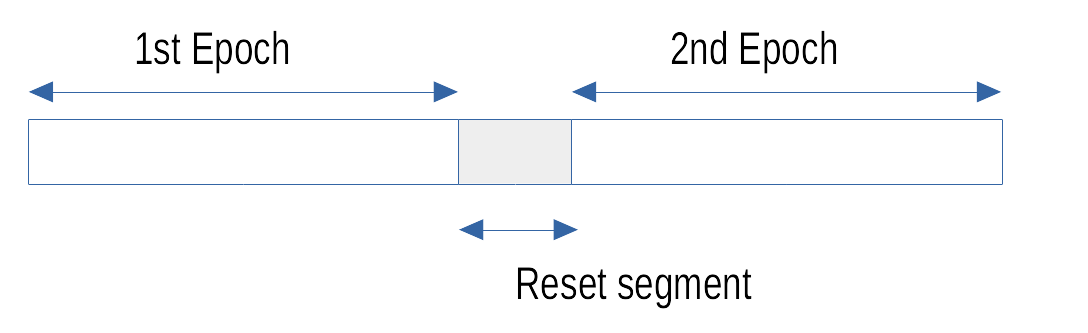
\includegraphics[width=0.8\textwidth]{img/epoch-concatenation}
  \caption{If the supervised learning is performed with different epoch of data, this is equivalent to a unique epoch, providing a reset segment of length $R$, the maximal recurrent range, is inserted before each new epoch. During reset segment, we set $\kappa_{nt}  = 0$.}
  \label{epoch-concatenation}
\end{figure}

One aspect of the estimation is related to robustness, i.e., being able to take into account the fact that errors and artifacts may occur in the learning set, implemented here as a M-estimator, i.e., not  a least-square function but another alternative cost function, with a smaller slope for higher values.

\subsubsection*{Considering static estimation.}

The present framework stands for dynamic estimation of a temporal sequence. It can also simply be applied to a static estimation at the final time step $T-1$ considering $\bar{o}_n(T-1)$ only the previous values $o_n(t)$ being unconstrained. In that case the value $T$ corresponds to the number of iteration to obtain the desired estimation. In a non-recurrent architecture this value is easy to derive from the architecture, it corresponds to the number of computation steps. In a recurrent architecture, the situation is more complex since computation loops have to converged, and the number of computation steps is an explicit parameter, unless the system is tuned to converge to a fixed point, while considering $T \rightarrow +\infty$ which is a rather straightforward extension of the present work.

\subsection*{Considering constrained architecture and weights values.}

It is precious to also introduce constraints on the connection weights. Typical constraints include: 
\\- sparse connectivity, which reduces the total amount of computation, and allows internal sub-assemblies to emerge, 
\\- positive or negative weight values (corresponding to excitatory or inhibitory connections).

The design choice of the kernels allows us to constraint the network connectivity. It is possible to specify partial connectivity allowing to distinguish different layers (e.g. hidden layers not connected to input and/or output).
This may be, for instance, a 2D-topography with local horizontal connections, or several layers with, e.g., either point to point, or divergent connectivity between layers.

However, if the architecture itself has to be learned, the present framework may be used in another way: Starting from a given connected network and performing a sparse estimation, may lead to a result with zero weight values for connections not present in the estimated architecture, and non zero values otherwise. This is a sparse estimation, i.e. not only minimizing the metric not only with respect to the weights values, but also with respect to the fact that some weights have either zero or non-zero values, i,e, with respect connection sets. Sparse estimation methods (see e.g. \cite{tropp:04a,tropp:04b} for a didactic introduction) can be used to this end. 

One application could be modulatory weighted connections, allowing to enhance or cancel sub-parts of the network connectivity.

In our case we may simply choose, for some meta-parameters $\nu_{nd}$: 
\[
{\cal R}({\bf W}) = \sum_{nd} \frac{\nu_{nd}}{\epsilon + |\hat{W}_{nd}|} \, W_{nd}^2
\]
where $\hat{W}_{nd}$ stands for the best a-priory or previous estimation of the weight. This leads to a reweighted least-square criterion, where small weights value minimization is reinforced, up to $0$, yielding sparse estimation.

The case where we consider excitatory or inhibitory connections (i.e., weight values that only positive or negative), or the case where the weights are bounded, is managed at the implementation level, as a hard constraint in the minimization. Very simply, if the value is beyond the bound it is reprojected on on the bound. This may lead to a sub-optimal estimation, but avoids the heavy management of Karush-Kuhn-Tucker conditions.

As an example, let us consider the adjustable leak $\gamma_{nt}$, $0 \leq \gamma_{nt} \leq 0.99 \simeq 1$ of a NLN unit. If the minimization process yields a negative value, the value is reset to zero (it means that we better have no leak). If the minimization process yields an unstable value higher than one, it is reset to, say, $0.99$ to be sure the system will not diverge.

\subsection*{Considering un-supervised regularization.}

In order to find an interesting solution, we have to constraint the hidden activity to be estimated. Interesting properties includes sparseness, orthogonality, robustness and bounds.

Sparse activity (i.e., with a maximal number of values closed or equal to zero), which is known to correspond to unit assemblies tuned to a given class of input statistics, can be specified as a reweighted least-square criterion again, for some meta-parameters $\kappa_{nd}$:
\[
\rho_{nt}(x_{nt}) = \frac{\kappa_{nd}}{\epsilon + |\hat{x}_{nt}|} \, x_{nt}^2
\]
where $\hat{x}_{nd}$ stands for the previous estimation, with an initial value equal to $\kappa_{nd}$.

Orthogonality of hidden unit activities, in order to avoid redundancy and maximize the dynamic space dimension in the recurrent network, can also be specified, the same way as :
\[
\rho_{nt}(x_{nt}) = \kappa_{nd} \, \sum_{n' \neq n} (\sum_t x_{nt} \, \hat{x}_{n't})^2
\]
again as as, now not local but global, reweighted least-square criterion, now minimizing the dot products between unit activities, thus minimal when orthogonal. 

Another aspect concerns the fact we may have to control the activity bound, e.g., a weak constraint of the form $x_{nt} \preceq b$. Following the same heuristic, we may introduce a cost of the form:
\[
\rho_{nt}(x_{nt}) = \kappa_{nd} \, e^{k\,(x_{nt} - b)}
\]
with $k > 0$ in order to have a fast increasing function as soon as the bound is violated.

\clearpage\section{Closed forms solution for neural network tasks} \label{closedforms}

Let us illustrate how the type of used units has a strong influence on the difficulty of the task. Here we consider deterministic tasks only. The remark is that tasks considered as quite complex \cite{Hochreiter:1997,Gers:2003,martens_learning_2016} for certain architectures are trivial for others. In particular, the use of AIF neurons simplifies certain problems, e.g. requiring long short-term memory. We illustrate this point here considering deterministic sequence generation and long-term non-linear transform, and provide explicit simple solutions for those problems.

\subsubsection*{Generating long term sequential signals}

The lever is that it is straightforward to generate a delayed step signal (i.e., equal to 0 before $t=\tau$, and 1 after) using AIF units, e.g.:
\eqline{s_\tau(t) = \frac{1}{2} \, (1 - \Upsilon(s_\tau(t-1))) \, s_\tau(t-1) + h_\tau}\\
with 
\eqline{h_\tau \deq \frac{1}{4\, \left(1 - 2^{\frac{1}{2}-\tau}\right)} \in [h_\infty = 1/4, h_1 \simeq 0.85],}\\  
for which we easily obtain\footnote{{\bf Delayed step signal.} Starting with $s_\tau(0) = 0$ this first order recurrent equation yields: 
\eqline{s_\tau(t) = 2 \, h \, \left(1 - 2^{-t}\right) \in [0, 2\, h],} 
which is an bounded increasing negative exponential profile, for which the parameter $h$ has been chosen to maintain $s_\tau(t) < 1/2, t < \tau$, and reach $s_\tau(t) > 1/2$, for $t \geq \tau$.
\hr} $\Upsilon(s_\tau(t)) = \delta_{t\geq\tau}$. 

The numerical limit of this method is the fact that for huge value of $\tau$ the parameter precision must be of order $O\left(2^{-\tau}\right)$. To avoid this constraint, either an architecture with several units building a delay line, or with a ramp unit and adaptive thresholds (see next section) can be considered.

From this basic element we can generate a delayed clock signal\footnote{{\bf Delayed clock signal.} Modifying the delayed step signal, and adding a memory carousel unit in order to reset the signal after the step and keep it reseted, we obtain: 
\eqline{\begin{array}{rcl}
 c_\tau(t) &=& \frac{1}{2} \, (1 - \Upsilon(c_\tau(t-1))) \, c_\tau(t-1) + h_\tau \, (1 - \Upsilon(d_\tau(t-1))) \\
 d_\tau(t) &=& d_\tau(t-1) + \Upsilon(c_\tau(t-1)), \\
\end{array}}
with $\Upsilon(c_\tau(t)) = d_\tau(t) = 0, t < \tau$, until $c_\tau(\tau) > 1/2$, As a consequence $d_\tau(\tau + 1) = 1$, thus $c_\tau(\tau + 1) = 0$, which is a stable fixed point, values remaining constant beyond. Finally we obtain $\Upsilon(c_\tau(t)) = \delta_{t=\tau}$ in this case.
\hr} or another long-term mechanism, such a as flip-flop\footnote{{\bf Defining a flip-flop latch.} Let us defined a SR-latch (i.e., a flip-flop) with:
\eqline{\begin{array}{rcl}
z(t) &=& \Upsilon(z(t-1)) + \Upsilon(i_1(t)) - \Upsilon(i_0(t))\\
\end{array}}
yielding the following behavior:
\\- {\em R-state}: If $i_0(t) < 1/2$ and $i_1(t) < 1/2$ (no-input) and $z(t-1) < 1/2$, then $z(t) = 0 < 1/2$, the reset state is maintained.
\\- {\em S-state}: If $i_0(t) < 1/2$ and $i_1(t) < 1/2$ (no-input) and $z(t-1) > 1/2$, then $z(t) = 1 > 1/2$, the set state is maintained.
\\- {\em R-S transition}: If $i_0(t) < 1/2$ and $i_1(t) > 1/2$  and $z(t-1) < 1/2$, then $z(t) = 1 > 1/2$, flipping to a set state; if it was already in the set state, we still have $z(t) = 2 > 1/2$.
\\- {\em S-R transition}:If $i_0(t) > 1/2$ and $i_1(t) < 1/2$  and $z(t-1) > 1/2$, then $z(t) = 0 < 1/2$, flipping to a reset state; f it was already in a reset state, we still have $z(t) = - 1 < 1/2$.
\\- {\em no instability}: $i_0(t) > 1/2$ and $i_1(t) > 1/2$ contrary to a standard digital RS-latch we simply have $z(t) = \Upsilon(z(t-1))$ providing it was in set of reset state, without any meta-stability.
\hr}, which is a fundamental building blocks of any digital transform, in conjunction with logic gates such as a xor gate\footnote{{\bf Defining the xor function.} It is straightforward to notice that: 
\eqline{\begin{array}{rcl}
x_\bullet(t) &=& \Upsilon(x_a(t - 1)) + \Upsilon(x_b(t - 1)) + -2 \, \Upsilon(x_o(t)) \\
x_o(t) &=& \Upsilon(x_a(t - 1)) + \Upsilon(x_b(t - 1)) - 1 \\
\end{array}}
verifies 
\eqline{\begin{array}{rcl}
\Upsilon(x_o(t))  &=& \Upsilon(x_a(t - 1)) \mbox{ and } \Upsilon(x_b(t - 1)) \\
\Upsilon(x_\bullet(t))  &=& \Upsilon(x_a(t - 1)) \mbox{ xor } \Upsilon(x_b(t - 1)) \\
\end{array},}
while other logic gates are easy to build in a similar manner.\\ A step further the expression 
\eqline{x_\dagger(t) = 1/2 - 2 \, (\Upsilon(x_a(t - 1)) - 1/2) \, (\Upsilon(x_b(t - 1)) - 1/2)}
now considering a multiplication unit, directly calculates the xor function, but does no correspond to some AIF unit.
\hr}. 

If we consider a mollification instead of a step function (i.e., replacing $\Upsilon$ with$\Upsilon_\epsilon$ in the previous equation), we obtain the behavior for sufficiently large slopes. More precisely\footnote{This is obtained, e.g., by the following piece of maple code: {\tt upsilon := (u) -> 1/(1+exp(-4*(u - 1/2)/epsilon)):\\
c\_n := c -> (1 - upsilon(c)) * c / 2 + h:\\
bounds := [solve(c\_n(1/2) = 1/2, h), solve(c\_n(0) = 1/2, h)];\\}\hr}, for instance, we numerically observed the same qualitative behavior in the delayed step signal case, with $h \in [h_\infty = 0.376, h_1 = 0.5]$, while $h$ is not given in closed form in this case.

Further on this track, it is clear that we can compile any sequential circuit in such networks, which is far from being new. The add-on here is about that the fact we provide explicit solutions, using AIF neurons, with a lower complexity in terms of network nodes than using LSTM units. Let us see two paradigms where this enlighten the problem complexity.

\subsubsection*{Long term non-linear transform}

In many experiments, a variant of a sequence of the form:
\\\centerline{\begin{tabular}{lcccccccccccc}
time :  & 0   & 1   &     &          &     & T\\
input:  & $a$ & $b$ & $*$ & $\cdots$ & $*$ & $*$\\
output: & $*$ & $*$ & $*$ & $\cdots$ & $*$ & $a \, b$ \\
\end{tabular}}\\
where $a$ and $b$ are variable input, $*$ are random distractors and $a\,b$ the desired delayed output (here a product, but it could be another calculation). Such setup combines several non-trivial aspects, long short term memory, distractor robustness, and operation which may not explicitly hardwired in the network, presently a product. The LSTM approach was shown to be particularly efficient for such computation, because of the notion of ``memory carousel''. In fact, the explicit implementation of such a mechanism on the given example is trivial\footnote{{\bf An example of long term computation.} One solution writes: 
\eqline{\begin{array}{rcl}
o_0(t) &=& (1 - \Upsilon(c_T(t)) \, i(t) + (\Upsilon(c_T(t)) - 1) \, x_a(t) \, x_b(t) + \\
x_a(t) &=& (1 - \Upsilon(c_0(t)) \, x_a(t-1) + (\Upsilon(c_0(t)) - 1) \, i(t) \\
x_b(t) &=& (1 - \Upsilon(c_1(t)) \, x_b(t-1) + (\Upsilon(c_1(t)) - 1) \, i(t) \\
\end{array}} 
while $c_\tau(t) = \delta_{t = \tau}$ are clock signals, as defined previously, and it is easy to verify that $x_a(t)$ ``opens'' the memory at time $t=0$, and stores the previous value otherwise, with a similar behavior for $x_b(t)$, while $o_0(t)$ simply mirror the input until $t=T$, where the expected result is output. Obviously, these are no more AIF units but introduce multiplications between state values}.

What do we learn from this very simple development? While authors have already made explicit the fact that such computations rely on ``gate unit'' and ``memory unit'', it seems that ``delayed unit'' (i.e. learning a time delay) are also basic components. It is also an example of how deterministic computations might become simple, if we introduce a-priory information on the computation, via dedicated units.

\subsubsection*{Deterministic sequence generation}

What is the complexity of the task of generating a deterministic time sequence $\bar{o}_n(t), n \in \{0, N_0\{, t \in \{0, T\{$, with a recurrent network of $N \ge N_0$ units of range $R$? This could be an unpredictable sequence, without any algorithm to generate it, unless copying all sample (i.e., with a maximal Kolmogorov complexity).

On one hand, $O(N_0)$ independent linear recurrent units of range $R=T$, solves the problem of generating an exact sequence of $N_0 \, T$ samples, in closed form\footnote{{\bf Long range sequence generation.} Let us consider units of the form:
\eqline{x_n(t) = \sum_{d = 1}^{d = T-1} W_{nd} \, x_n(t-d) + W_{n0},}
thus with $N_0 \, T$ weights. Since $x_n(t) = 0, t < 0$, providing $\bar{o}_n(1) \neq 0$, we immediately obtain $W_{n0} = \bar{o}_n(1)$ and for $d > 0$: 
\eqline{W_{nk} = (\bar{o}_n(k+1) - W_{n0} - \sum_{d = 1}^{d = k-1} W_{nd} \, \bar{o}_n(t-d)) / \bar{o}_n(1),}
providing that $\bar{o}_n(1) \neq 0$, thus a closed-form solution. If $\bar{o}_n(1) = 0$ we simply have to generate the sequence, say, $\bar{o}'_n(t) = \bar{o}_n(t) + 1$ and add a second unit of the form $x_n(t) = x'_n(t) - 1$, using now an additional node.
\hr}. This solution requires a very large recurrent range, and the numerical precision is limited by the fact that errors accumulate along the recurrent calculation.

On the other hand, feed-forward units of range $R=1$ solve explicitly the problem using $T$ clock units and $N_0$ readout units, with $O(N_0\,T)$ weights. This requires no more than $N_0+T$ units considering binary information\footnote{{\bf Long sequence generation with delay lines.} Let us consider $N_0$ readout units and $T$ clock units of the form: 
\eqline{\begin{array}{rcll}
x_{n_0}(t) &=& \sum_{n = 0}^{T-1} (\bar{o}_{n_0}(n) - \bar{o}_{n_0}(n+1)) \, \Upsilon(x_{N_0+n}(t)) & 0 \leq n_0 < N_0, \mbox{ writing }  \bar{o}_{n_0}(T) \deq 0\\
x_{N_0}(t) &=& \frac{1}{2} \, (1 - \Upsilon(x_{N_0}(t-1))) \, x_{N_0}(t-1) + h_1 \\
x_{N_0+n}(t) &=& x_{N_0+n-1}(t-1) & 0 < n < T \\
\end{array}}
thus providing $T$ delayed step signals such that $\Upsilon(x_{N_0+n}(t)) = \delta_{t>n}$, allowing us to generate the desired sequence combining these signals. If we now consider mollification of he threshold function, the previous system of equation is going to generate a temporal partition of unity. Since ${\bf x}_{N_0+n}$ are simple shifts of ${\bf x}_{N_0}$, the clock units obviously span the output signal space and output units can easily linearly adjust there related combination to obtain the desired values.
\hr}, and no more that $N_0+1$ units if the numerical precision is sufficient and unit threshold adjustable\footnote{{\bf Long sequence generation with a ramp unit.} If we can consider units of the form: 
\eqline{\begin{array}{rcrl}
x_{n_0}(t) &=& \sum_{n = 0}^{T-1} (\bar{o}_{n_0}(n) - \bar{o}_{n_0}(n+1)) \, \Upsilon(x_{N_0+n}(t) - \theta_n) \\
x_{N_0}(t) &=&  x_{N_0}(t-1) + 1\\
\end{array}}
with the ramp unit $x_{N_0}(t)$ precision being of order $O(1/T)$, while we now can introduce adaptive thresholds $\theta_n = n$, it is obvious to verify that we solve the problem with two units.
\hr}.
A step further, considering less than $N_\bullet \deq \sqrt{N_0\,T/R}$ linear or NLN units of range $R$, we can not generate a solution in the general case\footnote{{\bf Long sequence generation with fully connected network.} Considering the linear network system:
\eqline{x_n(t) = \sum_{m = 1}^{m  = N} W_{nmr} \sum_{r= 1}^{r=R} \, x_m(t-r) + W_{n0},}
with $0 \leq n_0 < N_0$ output units and $N_0 \leq n < N$ hidden units, using vectorial notations, with the shift operator ${\cal S}$ defined as ${\cal S} {\bf x}(t-1) = {\bf x}(t)$, we obtain:
\eqline{{\cal S} \, \begin{array}{r}{}_{N_0\,T}\updownarrow\\ {}_{(N-N_0)\,T}\updownarrow \end{array}
\left(\begin{array}{c} \bar{\bf o} \\ \bar{\bf x} \end{array}\right) = {\bf W} \, \left(\begin{array}{c} \bar{\bf o} \\ \bar{\bf x} \end{array}\right) + W_{0}}
where $\bar{\bf o}$ are the desired output. It is a bi-linear system of $N\,T$ equations in $N^2\,R + N$ independent unknowns, i.e., the weights, while the $(N-N_0)\,T$ hidden values are entirely specified as soon as the weights are given. In terms of number of degree of freedom we can not have $N^2\,R + N < N_0 \,T$ for this algebraic system of equation to have a solution in the general case.}.

The generation of periodic signal of period $T$, is a very similar problem, as studied in \cite{rostro-gonzalez-cessac-etal:10}, for $N=N_0$. In a nutshell, we simply must add equations such that ${\bf x}(T) = {\bf x}(0)$ to guaranty the periodicity.

From this discussion, we see that the complexity of signal generation problem highly depends on the kind of ``allowed units'' and reduces to a trivial problem as soon as suitable operation are allowed. Furthermore, there exist a $R=1$ network of at most $N_0 + T$ units that exactly solves the problem, without requiring huge precision, while a linear network, a NLN network or a AIF network can generate such a sequence in the general case, with either a closed form solution, or solving a linear system of equation.

\clearpage\section{Stochastic adjustment of the network weights}\label{stochastic}

Let us consider the problem of optimizing the probabilistic distribution $\tilde{p}(\tilde{\bf x} = {\bf x})$ of a network output, as a function of the desired distribution $\bar{p}(\bar{\bf o} = {\bf o})$ of a root network. Since we are in a multi-dimensional and dynamic framework, with continuous values, it is  intractable  to consider as it the distribution, but only a parametric model of it, and adjust the parameters of this model. 

\subsubsection*{An illustrative example}

Let us, for instance, consider that it is important that the network output mean $\tilde{\Omega}_{n,\bullet}$ and auto-correlation in a $\tau = \{0, \Delta\}$ time window $\tilde{\Omega}_{n,\tau}$, correspond to some desired values:
\eqline{\begin{array}{rclrcl}
   \bar{\Omega}_{n,\bullet}  &\deq& \frac{1}{T} \, \sum_{t = 0}^{T - 1} \omega_{n,\bullet}(t), & \omega_{n,\bullet}(t) &\deq& \bar{o}_n(t) \\
   \bar{\Omega}_{n,\tau}  &\deq& \frac{1}{T - \tau} \, \sum_{t = 0}^{T - \tau - 1} \omega_{n,\tau}(t) & \omega_{n,\tau}(t) &\deq& \bar{o}_n(t) \, \bar{o}_n(t - \tau), \\
\end{array}}
the normalized temporal auto-correlation being: 
\eqline{C_{n,\tau} = (\bar{\Omega}_{n,\tau} - \bar{\Omega}_{n,\bullet}^2) / (\bar{\Omega}_{0,\tau} - \bar{\Omega}_{n,\bullet}^2).}
We thus do not constraint the output desired values directly but only some momenta expectation.

Beyond this example, we thus consider observable $\omega_{k}(x_n(t) \cdots x_n(t-\tau_k))$ of a given rank $\tau_k$ and their expectation on the desired distribution $\Omega_{k}$. We could also have considered higher order momenta, e.g., consider mean, standard-deviation, skewness and kurtosis, or spatial correlations, and so on.

\subsubsection*{Considering a general model}

Adapting the development given in \cite{vasquez:inria-00574954} for binary distribution, we propose to minimize the KL-divergence, considering maximal entropy Gibbs distributions. We are going to propose to adjust the network weights in order to minimize an approximation of the KL-divergence between the desired and simulated distribution.

If we look for a distribution of probability with maximal entropy and which observable $\omega_{k}$ correspond to some expectation values ${\Omega}_{k}$, we obtain:
\eqline{p({\bf x}) = \frac{\exp\left(\sum_k \lambda_k \, {\omega}_{k}({\bf x}) \right)}{Z_p({\bf \lambda})},}
where the denominator guaranties $\int_{{\bf x}} p({\bf x}) = 1$ and is called the partition function\footnote{{\bf Maximal entropy distribution.} Given expectation  ${\Omega}_{k}$  of observable $\omega_{k}(t)$ we state that we look for a probability distribution of maximal entropy which corresponds to the observable expectation. This writes, with Lagrangian multipliers $\lambda_k$:
\eqline{\min_{\bf \lambda} 
\underbrace{\int_{\bf x} p({\bf x}) \log(p({\bf x}))}_{entropy} +
\underbrace{\lambda_{0} \left(\int_{\bf x} p({\bf x}) -1 \right)}_{normalization} -
\underbrace{\sum_k \lambda_{k} \left(\int_{\bf x} p({\bf x}) \, \omega_{k} - {\Omega}_{k}\right)}_{observations}}
and the functional derivative of this criterion yields:
\eqline{p({\bf x}) = \exp\left(\sum_k \lambda_k \, {\omega}_{k}({\bf x})\right) / Z_p({\bf \lambda}),}
as easily obtained from the normal equation derivation, see e.g.:
\\ \centerline{\href{https://en.wikipedia.org/wiki/Maximum\_entropy\_probability\_distribution\#Proof}{https://en.wikipedia.org/wiki/Maximum\_entropy\_probability\_distribution\#Proof}.}\hr}, topological pressure or free energy. The quantity $Z_p({\bf \lambda})$ has no closed form beyond simple cases, and can be numerically estimated as:
\eqline{Z_p({\bf \lambda}) = \int_{\bf x} \exp\left(\sum_k \lambda_k \, {\omega}_{k}({\bf x})\right) \simeq \frac{1}{T - \tau} \, \sum_{t = 0}^{T- \tau} \exp\left(\sum_k \lambda_k \, {\omega}_{k}(t)\right)}, under the ergodic assumption, $\tau$ being chosen for all observable ${\omega}_{k}(t)$ to be defined.

\subsubsection*{Fitting a Gibbs distribution}

A step further, it appears that minimizing the KL-divergence between the observed distribution $\bar{p}(\bar{\bf o})$ and the Gibbs model corresponds to adjust the parameters $\bar{\bf \lambda}$ in order the predicted observable expectation $\Omega_k({\bf \lambda})$ to get as closed as possible to the desired observable expectation $\bar{\Omega}_{k}$, which is a standard estimation problem (in a nutshell, the trick is to minimize the criterion gradient, not the criterion itself\footnote{{\bf Fitting the Gibbs parameters distribution}. For the sake of completeness, let us detail how such estimation can be performed. If we consider the KL-divergence between the observed distribution $\bar{p}(\bar{\bf o})$ and the model approximate distribution $q({\bf x}))$, we easily derive: 
\eqline{\begin{array}{rcl}
d_{KL}(\bar{p}(\bar{\bf o})\|q({\bf x})) 
&=& \int \bar{p}(\bar{\bf o}) \, \log\left(\frac{\bar{p}(\bar{\bf o})}{q({\bf x})}\right) \\
&=& \int \bar{p}(\bar{\bf o}) \, \log\left(\bar{p}(\bar{\bf o})\right) - \int \bar{p}(\bar{\bf o}) \, \log\left(q({\bf x})\right) \\
&=& -h_{\bar{\bf o}} - \int \bar{p}(\bar{\bf o}) \log\left(q({\bf x})\right) \\
&=& -h_{\bar{\bf o}} - \int \bar{p}(\bar{\bf o}) \left(\sum_k \lambda_k \, \omega_{k} - \log(Z({\bf \lambda})) \right) \\
&=& -h_{\bar{\bf o}} - \sum_k \lambda_k \, \bar{\Omega}_{k} + 1 \, \log(Z_q({\bf \lambda})) \\
\end{array}}
combining the previous equations, and since the term $h_{\bar{\bf o}} \deq -\int \bar{p}(\bar{\bf o}) \log(\bar{p}(\bar{\bf o}))$ is the observed entropy and is constant with respect to the parameter to estimate, we are left with the following criterion, which in fact corresponds to cross-entropy maximization $\min_{\bf \lambda} {\cal J}$, with: 
\eqline{\begin{array}{rcl}
 {\cal J} &=& \log\left(Z_q({\bf \lambda})\right) - \sum_k \lambda_k \, \bar{\Omega}_{k} \\
 \partial_{\lambda_k} {\cal J} &=& \Omega_k({\bf \lambda}) - \bar{\Omega}_{k} \\
 \partial_{\lambda_k\, \lambda_l} {\cal J} &=& \Omega_{kl}({\bf \lambda}) \\
\end{array}}
writing $\omega_{kl}(t) = \omega_k(t) \, \omega_l(t)$, and $\Omega_{kl} = {\mathbb E}[\omega_{kl}]$. This computation comes from the fact that:
\eqline{\begin{array}{rcl}
Z_q({\bf \lambda}) 
&=& \int_{{\bf x}} \exp\left(\sum_k \lambda_k \, {\omega}_{k}({\bf x}) \right) \\
\partial_{\lambda_k} Z_q({\bf \lambda}) 
&=& \int_{{\bf x}} \exp\left(\sum_k \lambda_k \, {\omega}_{k}({\bf x}) \right) \, {\omega}_{k}({\bf x}) \\
&=& \int_{{\bf x}} Z_q({\bf \lambda}) \, q({\bf x}) \, {\omega}_{k}({\bf x}) \\
&=& Z_q({\bf \lambda}) \, {\Omega}_{k}({\bf \lambda}),
\end{array}}
and it is easy to approximate:
\eqline{\begin{array}{lrcl}  
\Omega_{l}({\bf \lambda}) 
&\deq& \int_{\bf x} \frac{\exp\left(\sum_k \lambda_k \, \omega_{k}\right)}{Z_q({\bf \lambda})} \omega_l(t)\\
&\simeq& \frac{1}{T - \tau_l} \, \sum_t \omega_l(t) \\
\end{array}}
under the ergodic assumption.

As a consequence, despite the caveat that $Z_q({\bf \lambda})$ calculation is usually not tractable, this allows us to implement some paradigm that tends to minimize the criterion gradient (since at a criterion minimum, the gradient vanishes):
\eqline{\bar{\lambda} = \mbox{arg min}_\lambda |\Omega_{l}({\bf \lambda}) - \bar{\Omega}_{k} |.}
One example of algorithm writes:
\\ \hphantom{2mm} {\em Input} : The desired observable values $\bar{\Omega}_{k}$ and the distribution samples $\bar{\bf o}$.
\\ \hphantom{2mm} {\em Output} : The estimated $\bar{\lambda}_k$.
\\ \hphantom{4mm} - Starts with ${\bf \lambda}_0 = 0$ and a regularization parameter $\upsilon = 1$.
\\ \hphantom{4mm} - At a given iteration $i$
\\ \hphantom{4mm} -- Computes $\Omega_k({\bf \lambda})$ and $\Omega_{kl}({\bf \lambda})$ for a given value of ${\bf \lambda}$ from a random draw $\pi(t)$.
\\ \hphantom{4mm} -- In order to obtain ${\bf \lambda}_{i} = d{\bf \lambda} + {\bf \lambda}_{i-1}$ solve the regularized linear problem: 
\eqline{d{\bf \lambda} = \mbox{arg min}_{d{\bf \lambda}} |d{\bf \lambda}|, \;\;\; \upsilon \, \partial {\cal J} + (1 - \upsilon) \, \partial^2 {\cal J} \, {\bf \lambda}_{i-1} = \partial^2 {\cal J} \, d{\bf \lambda}}
calculating the SVD of $\partial^2 {\cal J}$ in order to consider its pseudo-inverse.
\\ \hphantom{4mm} -- If $\|\partial {\cal J}\|$ does not decreases reduce $\upsilon$ and repeat until $\upsilon$ vanishes.
\hr}). As a consequence, given a desired output $\bar{\bf o}$ and a choice of observable $\omega_k$ we can estimate the maximal entropy parameters $\bar{\bf \lambda}$.

\subsubsection*{Statistical weight adjustment from the parametric model}

Given set of desired observable values $\bar{\Omega}_k$, with the corresponding Gibbs model $\hat{p}(\bar{\bf o})$ parameterized by $\bar{\bf \lambda}$ and adjusted on the reference samples $\bar{\bf o}$, we now can state the problem of adjusting the network weights. We consider the KL-divergence between the observed distribution $\bar{p}(\bar{\bf o})$, approximated by the related Gibbs model, and the network simulation $\tilde{p}_{\bf W}(\tilde{\bf x})$, parameterized by the network weights ${\bf W}$. The network is viewed here as a parametric model of the observed distribution. 

Since the network simulation is brought to the desired reference samples distribution, modeled as a Gibbs distribution, we are going to assume that the network simulation can itself be represented by a Gibbs distribution:
\eqline{\tilde{p}(\tilde{\bf x}) \simeq \exp\left(\sum_k \tilde{\lambda}_k \, {\omega}_{k}({\bf x})\right) / Z_{\tilde{p}}(\tilde{\bf \lambda}),}
yielding, using similar algebra as before:
\eqline{\begin{array}{rcl} d_{KL}(\bar{p}(\bar{\bf o})\|\tilde{p}(\tilde{\bf x})) 
 &=& \int p(\bar{\bf o}) \log\left(\frac{\bar{p}(\bar{\bf o})}{\tilde{p}(\tilde{\bf x})}\right) \\
 &\simeq& \int p(\bar{\bf o}) \log\left(\frac{\hat{p}(\bar{\bf o})}{\tilde{p}(\tilde{\bf x})}\right) \\ &=& \sum_k (\bar{\lambda}_k - \tilde{\lambda}_k) \, \bar{\Omega}_{k}
          + \log(Z_{\tilde{p}}(\tilde{\bf \lambda})/Z_{\bar{p}}(\bar{\bf \lambda})) \\
\end{array}}
with the goal to adjust the weights in order the related $\tilde{\bf \lambda}$ to minimize this divergence. As before, we can replace the KL-divergence minimization by the minimization of the gradient magnitude. This design choice is valid because the topological pressure is convex with respect to ${\bf \lambda}$, so that the criterion is convex \cite{vasquez:inria-00574954}. As a consequence, the criterion is minimal when the gradient magnitude vanishes, i.e. is minimal too, while the criterion decreases with the gradient magnitude, thanks to being a convex criterion.

The gradient writes $\partial_{\tilde{\lambda}_k} d_{KL}(\bar{p}(\bar{\bf o})\|\tilde{p}(\tilde{\bf x})) = \tilde{\Omega}_{k}(\tilde{\bf \lambda}_{\bf W}) - \bar{\Omega}_{k}$, and we propose to consider the following weighted ${\cal L}^1$ norm:
\begin{equation} \label{kl-criterion} \rho({\bf x}) \deq \sum_k |\bar{\lambda}_k| \, \left|\bar{\Omega}_{k} - \frac{1}{T-\tau_k} \sum_t \omega_k(t)\right|. \end{equation}
The reason of this second design choice is that it has the same order of magnitude as the $d_{KL}(\bar{p}(\bar{\bf o})\|\tilde{p}(\tilde{\bf x}))$ with respect to the observable, i.e.:
\eqline{|\partial_{\bar{\Omega}_k} d_{KL}(\bar{p}(\bar{\bf o})\|\tilde{p}(\tilde{\bf x}))| = |\partial_{\bar{\Omega}_k} \rho({\bf x})| = |\bar{\lambda}_k|,}
so that we expect the numerical condition of the original criterion and the related gradient magnitude to be similar. At the experimental level we have observed that such ${\cal L}^1$ criterion seems more efficient than the corresponding ${\cal L}^2$ criterion.

\subsubsection*{Boostrapping the network estimation}

Given the previous criterion, we consider a network simulation $x_n(t)$, with the goal to modify the related network weights in order the network output observable to be $\frac{1}{T-\tau_k} \sum_t \omega_k(t)$ to be as closed as possible to the desired observable $\bar{\Omega}_k$. To this end, we define desired values $\hat{x}_n(t)$, as follows
\eqline{\min_{\hat{x}_n(t)} \frac{1}{2} \, \sum_{nt} (\hat{x}_n(t) - x_n(t))^2 + \sum_k \lambda_k \left[\bar{\Omega}_{k} - \frac{1}{T-\tau_k} \sum_t \left. \omega_k(t)\right|_{\hat{x}} \right]}
in words: The desired values are the closest values with respect to the present simulation that match the desired observable, while the normal equations yield the recurrent equation:
\eqline{\begin{array}{rcl}
  \hat{x}_n(t) &\leftarrow& x_n(t) + \sum_k \frac{1}{T-\tau_k} \, \lambda_k \, \sum_t \partial_{x_n(t)} \omega_k(t) \\
  \lambda_k &\simeq& \left[ \frac{1}{T-\tau_k} \, \frac{1}{T-\tau_{k'}} \, \sum_{nt} \partial_{x_n(t)} \omega_{k'}(t) \, \partial_{x_n(t)} \omega_{k}(t)^T \right]^{\dagger} \, \left[\bar{\Omega}_{k'} - \frac{1}{T-\tau_k'} \sum_t \omega_{k'}(t)\right] \\
\end{array}}
which is a standard non-linear constrained least-square 2nd order recurrent scheme (see e.g., \cite{vieville:inria-00074888}). In other words, we iteratively compute the projection $\hat{x}_n(t)$ of the present simulation $x_n(t)$ onto the manifold defined by $\bar{\Omega}_{k} = \frac{1}{T-\tau_k} \sum_t \omega_k(t)$, i.e., such that the desired values observables equal the desired observable values. Here, $\partial_{\bf x} \omega_{k}(t)$ corresponds to the local normal of the manifold, and since observables are mainly monomials of degree less than $D$, we can write for some $u_{nt} \in \{0, 1\}, d_{nt} \in \{0, D\}$ defining the monomial:
\eqline{\omega_{k}(t) = \prod_{nt} u_{nt} \, x_{n}(t)^{d_{nt}}, \mbox{ yielding } \partial_{x_{n't'}} \omega_k(t) = d_{n't'} \, \frac{\omega_{k}(t)}{x_{n't'}}}
which is well-defined, including for $x_{n't'} = 0$.

Such desired values may be used to provide local solutions to the estimation problem.



\clearpage{\scriptsize \bibliographystyle{plain} \bibliography{../etc/main,../etc/from-keops,../etc/from-sophia}}
\tableofcontents
\iffalse
\fi

\end{document}

